

 \documentclass[utf8x, 12pt]{G7-32} 

\usepackage{amsmath}

\DeclareMathOperator*{\argmin}{arg\,min}
\DeclareMathOperator*{\argmax}{arg\,max}

\sloppy

% Настройки стиля ГОСТ 7-32
% Для начала определяем, хотим мы или нет, чтобы рисунки и таблицы нумеровались в пределах раздела, или нам нужна сквозная нумерация.
\EqInChapter % формулы будут нумероваться в пределах раздела
\TableInChapter % таблицы будут нумероваться в пределах раздела
\PicInChapter % рисунки будут нумероваться в пределах раздела

% Добавляем гипертекстовое оглавление в PDF
\usepackage[
bookmarks=true, colorlinks=true, unicode=true,
urlcolor=black,linkcolor=black, anchorcolor=black,
citecolor=black, menucolor=black, filecolor=black,
]{hyperref}

% Изменение начертания шрифта --- после чего выглядит таймсоподобно.
% apt-get install scalable-cyrfonts-tex

% \IfFileExists{cyrtimes.sty}
%     {
%         \usepackage{cyrtimespatched}
%     }
%     {
%         % А если Times нету, то будет CM...
%     }

\usepackage{graphicx}   % Пакет для включения рисунков

\graphicspath{{assets/}}

% С такими оно полями оно работает по-умолчанию:
% \RequirePackage[left=20mm,right=10mm,top=20mm,bottom=20mm,headsep=0pt]{geometry}
% Если вас тошнит от поля в 10мм --- увеличивайте до 20-ти, ну и про переплёт не забывайте:
\geometry{right=20mm}
\geometry{left=30mm}


% Пакет Tikz
\usepackage{tikz}
\usetikzlibrary{arrows,positioning,shadows}

% Произвольная нумерация списков.
\usepackage{enumerate}

\usepackage{hyperref}
\definecolor{linkcolor}{HTML}{0000FF} % цвет ссылок
\definecolor{urlcolor}{HTML}{0000FF} % цвет гиперссылок
 
\hypersetup{pdfstartview=FitH,  linkcolor=linkcolor,urlcolor=urlcolor, colorlinks=true}

% ячейки в несколько строчек
\usepackage{multirow}

% itemize внутри tabular
\usepackage{paralist,array}

% Центрирование подписей к плавающим окружениям
\usepackage[justification=centering]{caption}

% 8 Листинги

\usepackage{listings}

% Значения по умолчанию
\lstset{
  basicstyle= \footnotesize,
  breakatwhitespace=true,% разрыв строк только на whitespacce
  breaklines=true,       % переносить длинные строки
%   captionpos=b,          % подписи снизу -- вроде не надо
  inputencoding=utf8x,
  extendedchars=false,
  keepspaces=true,
  numbers=left,          % нумерация слева
  numberstyle=\footnotesize,
  showspaces=false,      % показывать пробелы подчеркиваниями -- идиотизм 70-х годов
  showstringspaces=false,
  showtabs=false,        % и табы тоже
  stepnumber=1,
  tabsize=4,              % кому нужны табы по 8 символов?
  frame=single
}

% Стиль для псевдокода: строчки обычно короткие, поэтому размер шрифта побольше
\lstdefinestyle{pseudocode}{
  basicstyle=\small,
  keywordstyle=\color{black}\bfseries\underbar,
  language=Pseudocode,
  numberstyle=\footnotesize,
  commentstyle=\footnotesize\it
}

% Стиль для обычного кода: маленький шрифт
\lstdefinestyle{realcode}{
  basicstyle=\scriptsize,
  numberstyle=\footnotesize
}

% Стиль для коротких кусков обычного кода: средний шрифт
\lstdefinestyle{simplecode}{
  basicstyle=\footnotesize,
  numberstyle=\footnotesize
}

% Стиль для BNF
\lstdefinestyle{grammar}{
  basicstyle=\footnotesize,
  numberstyle=\footnotesize,
  stringstyle=\bfseries\ttfamily,
  language=BNF
}

% Определим свой язык для написания псевдокодов на основе Python
\lstdefinelanguage[]{Pseudocode}[]{Python}{
  morekeywords={each,empty,wait,do},% ключевые слова добавлять сюда
  morecomment=[s]{\{}{\}},% комменты {а-ля Pascal} смотрятся нагляднее
  literate=% а сюда добавлять операторы, которые хотите отображать как мат. символы
    {->}{\ensuremath{$\rightarrow$}~}2%
    {<-}{\ensuremath{$\leftarrow$}~}2%
    {:=}{\ensuremath{$\leftarrow$}~}2%
    {<--}{\ensuremath{$\Longleftarrow$}~}2%
}[keywords,comments]

% Свой язык для задания грамматик в BNF
\lstdefinelanguage[]{BNF}[]{}{
  morekeywords={},
  morecomment=[s]{@}{@},
  morestring=[b]",%
  literate=%
    {->}{\ensuremath{$\rightarrow$}~}2%
    {*}{\ensuremath{$^*$}~}2%
    {+}{\ensuremath{$^+$}~}2%
    {|}{\ensuremath{$|$}~}2%
}[keywords,comments,strings]

\lstdefinelanguage[]{sqlite}[]{sql}{
  deletekeywords={POSITION},
  morekeywords={total},
  commentstyle=\color{gray}
}

\lstdefinelanguage[]{sql-explain}[]{sqlite}{
  morekeywords={SCAN, SEARCH},
  breaklines=false
}

% Подписи к листингам на русском языке.
\renewcommand\lstlistingname{\cyr\CYRL\cyri\cyrs\cyrt\cyri\cyrn\cyrg}
\renewcommand\lstlistlistingname{\cyr\CYRL\cyri\cyrs\cyrt\cyri\cyrn\cyrg\cyri}

% Любимые команды
\newcommand{\Code}[1]{\textbf{#1}}


\begin{document}

\frontmatter 

\newcommand{\HRule}{\rule{\linewidth}{0.5mm}}

\begin{center}

\textsc{Министерство образования и науки Российской Федерации
Федеральное государственное бюджетное образовательное учреждение 
высшего профессионального образования}\\[0.5cm]

\textsc{\large Московский государственный технический университет имени Н.\,Э.~Баумана}\\
\textsc{(МГТУ им. Н.Э.Баумана)}\\[0.5cm]

\includegraphics[scale=0.5]{bmstu-logo.png}~\\

\textsc{Факультет <<Информатика и системы управления>>}\\
\textsc{Кафедра <<Программное обеспечение ЭВМ\\и информационные технологии>>}\\[1cm]


\textsc{\huge Расчётно-пояснительная записка}\\
\textsc{\largeк дипломному проекту}\\
\textsc{на тему}\\

\HRule \\[0.5cm]
{\huge \bfseries Рекомендательная система развития городских анклавов}
\HRule \\[0.5cm]

\vfill

\begin{flushright}
  \begin{tabular}{rrlc}
    Исполнитель:  &    студент ИУ7-47и & Андино~Л.\,Г.  & \underline{\hspace{3cm}} \\[1cm]
    Руководитель: & преподаватель ИУ7 & Горин~С.\,В. & \underline{\hspace{3cm}} \\[1cm]
  \end{tabular}
\end{flushright}

{\large Москва, \the\year}

\end{center}

\pagenumbering{gobble}
\newpage
\pagenumbering{arabic}

\tableofcontents
\setcounter{page}{3}
\Introduction

Прежде всего, я благодарен за предоставленную возможность учиться в университете Баумана в Москве, особенно учителей  для получения образования, и за большое терпение у них с иностранными студентами, другим властям Университета, сотрудники деканата и другие чиновники, которые сделали и способствовали моему опыту, были лучшими. Я также хотел бы поблагодарить Министерство образования России за предоставленную возможность и российскую общину в целом за то, что у меня была возможность встретиться.

В настоящее время разработка и \textbf{Рекомендальная Система} или «RS» - это многодисциплинарные усилия, которые выиграли от результатов, полученных в различных областях компьютерных наук, в особенности машинного обучения и интеллектуального анализа данных, поиска информации и взаимодействия человека и компьютера. Между машинным обучением и интеллектуальным анализом данных существуют четкие отношения как подполя искусственного интеллекта, которые позволяют компьютеру научиться оптимально выполнять определенную задачу с использованием примеров, данных или прошлого опыта.

Например, «Data mining» \cite{data_mining}можно использовать для изучения данных транзакций у клиентов, которые купили «джинсы», также купили «футболки». Следовательно, рекомендации могут быть построены с использованием информации, предоставленной этими ассоциациями. Актуальные темы сосредоточены на использовании различных алгоритмов машинного обучения и «интеллектуального анализа данных» для прогнозирования пользовательских оценок для элементов или для обучения правильному ранжированию элементов для пользователя.

Двумя наиболее важными типами «RS» являются: «контент-основанный» и «комбинированная фильтрация». Рекомендатор «Content-based», который пытается порекомендовать элементы, подобные тем, которые были у других пользователей, понравился в прошлом, тогда как «Colaborative filtering» - это метод автоматического прогнозирования (фильтрации) интересов пользователя путем сбора предпочтений или информации о вкусах от многие пользователи (сотрудничающие). Основополагающее предположение подхода «Коллаборативная фильтрация» заключается в том, что если лицо «А» имеет такое же мнение, как лицо «В» по эмиссии, «А» с большей вероятностью имеет мнение «Б» по другой эмиссии, случайно выбранного человека.

В другой стороне отдельных систем рекомендаций может случиться так, что рекомендации могут иметь отношение к группе пользователей, а не к индивидууму \cite{porsuit}. 



В рекомендательной системе, ориентированной на отдельных лиц, нас интересует только максимальная индивидуальная удовлетворенность, и для этого достаточно всегда рекомендовать элемент с наивысшим рейтингом. Таким образом, нет необходимости точно прогнозировать удовлетворение. Однако, если мы заинтересованы в поддержании удовлетворенности группы, то внезапно становится более важно точно предсказать индивидуальное удовлетворение.

Чтобы остальная часть группы была счастлива, человеку, возможно, придется иногда сталкиваться с предметами, которые им не нравятся. Поэтому важно знать, не выбрали ли выбранные предметы не слишком неудовлетворенность отдельных лиц. Точные прогнозы индивидуальной удовлетворенности также могут помочь оценить стратегии адаптации групп.


В настоящее время индустрия сосредоточена на разработке надежных алгоритмов, которые могут дать надежные рекомендации, более сложные для злонамеренных пользователей, а также о том, что в алгоритмах используется масштабируемость для работы в больших наборах данных. Фактически, системы совместных рекомендаций зависят от доброй воли своих пользователей с неявным состоянием. И наоборот, академики ищут проблемы, которые могут быть решены в рамках научного сообщества. Это сделало и затруднит отраслевое и академическое сотрудничество.

Исследования выиграли от совокупного интереса и усилий, которые промышленность и научные круги имеют, но таким же образом требуют новых конкретных задач, и существует риск застоя, если мы не сможем решить полезные, но рискованные задачи в пользу проблем.

Основываясь на теории «разбитых окон» \cite{brokenw}, которая предполагает, что видимые признаки пренебрежения и плохого обслуживания в условиях окружающей среды поощряют преступность и беспорядок, в том числе серьезные преступления. Предложение начинается с прототипа программного обеспечения, разрабатывает модель, которая может быть использована в качестве развития кварталов, основанная на этих фактах: при разработке соседства существуют другие районы, уже разработанные в определенной области, которые содержат полезные данные, которые могут использоваться как рекомендации (видимые улучшения дома, культурные предложения и события и эволюция окрестностей). Если можно дать рекомендации для соседей, примените их к своим домам и рекреационной жизни, в результате общая окружающая среда получит качественное обновление. Пара проектов \cite{oregon}\cite{nextdoor} намерена развивать окрестности, но без поддержки RS до сих пор.


\textbf{Постановка задачи} Будет разработана рекомендательная система  для выбора продуктов для дома и рекреационных или культурных мероприятий, людьми, которые живут в определенном районе.  Исследование дополняется исследованиями и разработкой инструмента, в котором использование информации из системы рекомендаций по потребительским привычкам и возможное включение экспертных предложений может предоставлять неавтоматические рекомендации с целью предоставления преимуществ для как в обществе, в котором они живут.

Оценка этих рекомендаций исходит из сопоставления городского анклава, который хочет спровоцировать позитивные изменения, с другим городским анклавом, который был квалифицирован как удовлетворительный, хороший или превосходный в сравниваемом предмете.

В основном в двух областях вам необходимо получить рекомендации: рекомендации по приобретению товаров и / или мероприятий по благоустройству дома и рекомендации по рекреационной деятельности. На оба они, возможно, повлияли на добавление политик, установленных экспертами в каждой области.


Для достижения этой цели необходимо решить следующие задачи:


\begin{itemize}
\item Проведите анализ соответствующего метода фильтрации рекомендаций для каждой группы; необходимо будет проанализировать альтернативы алгоритмов, сравнивая их с соответствующими метриками;
\item В случае действий или рекомендаций, которые включают в себя ряд этапов, которые должны быть завершены, определите подходящий метод, который будет использоваться, оценивая доступные альтернативы;
\item Когда в рекомендациях, касающихся деятельности, участвует группа людей, будет определен способ установления удовлетворенности групп соответствующими методами;
\item Включение механизм логического вывода для определения рекомендаций для развития городских анклавов. Необходимые правила для включения рекомендаций начинаются с установленного уровня удовлетворенности, первоначально оцениваемого, но который может быть скорректирован с учетом обратной связи с окружающей средой и знаний экспертов в каждой области;
\item Чтобы оценить положительную оценку конкретного района, активность и удовлетворенность его жителей в отношении определенного Установить в эмпирическом масштабе, что считается развитым рядом в предметах, подлежащих изучению. Если это необходимо, сообщите другим заинтересованным сторонам, о квалификации, достигнутой развитыми секторами, и определите план, который потребуется для его достижения (действий);
\item Включить модуль для уведомления о рекомендациях в автономном режиме, когда необходимо отправить их пользователям соответствующей системы;
\item Убедитесь, что разработанные методы дают приемлемые решения;

\end{itemize}

\textbf{\textit{"Цель этой работы заключается в том, что из понимания математических и алгоритмических оснований модели «один к одному» или «поставщик-клиент», типичной для системы рекомендаций, разработан инструмент, который включает такие методы для приобретения товаров, но с добавлением других, которые сотрудничают в общем улучшении среды, в которой живут эти пользователи."}}












\mainmatter

\chapter{АНАЛИТИЧЕСКИЙ РАЗДЕЛ}
В разных разделах этой главы он использует отзывы пользователей, чтобы принимать решения об изменении при представлении предложений. Как читать эту главу: В разделе 1.1 представлена функциональная схема системы: типичный системный модуль рекомендации, модуль управления новыми идеями для совместной экономики и развития района и города.

В разделе 1.2 приводится краткий обзор того, какая система рекомендаций по использованию и приобретению товаров и услуг для домашнего благоустройства, выставок и культурных мероприятий. Математическая формулировка и показатели, доступные для оценки производительности.

В разделе 1.3 сначала анализируется подход «Совместная фильтрация», в котором подчеркиваются его характеристики, сильные и слабые стороны, и таким же образом с подходом, основанным на содержании, один из двух будет принят.

В разделе 1.4 анализируются альтернативы, которые возникают в результате улучшений, применяемых к районам, по сравнению с более развитыми в данной области, а также возможности для улучшения с точки зрения лучшего предложения или с учетом рекомендаций раздела 1.5 о совместной экономике и краудсорсинге через вклад жителей. Наконец, разделы 1.6 и 1.7 касаются модуля отчетов о проблемах города, в которых жители сообщают об инцидентах, и идеи, которые они могут внести в интересах развития города.


\section{Функциональная схема модели}
Выделяется модуль типичной системы рекомендаций, модуль управления новыми идеями для совместной экономики и развития района и города.

Поиск способов улучшения жилых районов начинается с анализа привычек потребления групп, проживающих в определенных городских анклавах, в соответствии с сбором информации из системы рекомендаций по купле-продаже по двум конкретным предметам. Первая группа занимается предметами благоустройства дома: садово-парковые изделия, растения и цветы, картины для дома и мебели. В то время как вторая касается предложений культурной и развлекательной деятельности.

Впоследствии оцениваются степень эволюции данного района как взвешивания суммы всего движения или деятельности как группы, а сравнения с другими соседями проводятся с целью внесения изменений или предложений по улучшению.

Впоследствии оцениваются степень эволюции данного района как взвешивания суммы всего движения или деятельности в качестве группы, и проводится сравнение с другими районами с целью внесения изменений или предложений по улучшению.

Возможность внесения улучшений может быть сделана после сопоставления кварталов и, например, для определения того, нужно ли это, чтобы улучшить предложение, добавить центры распределения или стимулировать потребление посредством рекламных акций или через «совместное потребление», поддержка «идей и решения» дается также системой.

\begin{figure}[h]
  \centering
  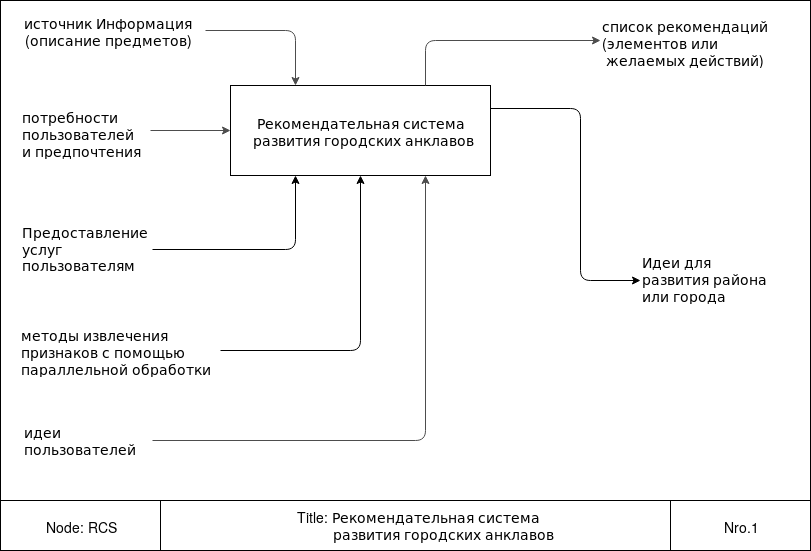
\includegraphics[scale=0.5]{diag1.png}
  \caption{Функциональная схема модели}
  \label{image:scheme3}
\end{figure}

\begin{figure}[h]
  \centering
  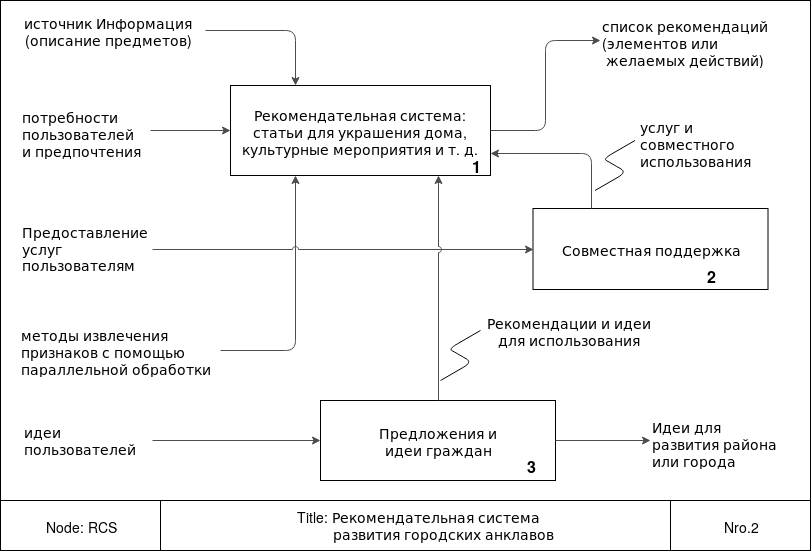
\includegraphics[scale=0.5]{diag2.png}
  \caption{Функциональная схема модели}
  \label{image:4}
\end{figure}
\hfill \break


\subsection{Лучшее использование отзывов пользователей}
Необходимо, чтобы люди получали рекомендации. Случай получения «ранжирования предметов» уже недостаточно. Кроме того, сайты рекомендаций не хотят делиться отзывами с третьими лицами. Система рекомендаций, которая управляет данными профиля пользователя, но может делиться отзывами с другими аналогичными системами с целью содействия сообществам.

Хорошо используемая обратная связь - это сила клиента, которая приносит пользу сообществу. С лучшей поддержкой мы будем стремиться содействовать развитию сообществ.

\begin{table}[]
\centering
\begin{tabular}{|p{2cm}|p{6cm}|p{6cm}|}
\hline
\multicolumn{3}{|p{14cm}|}{Классификация отзывов пользователей в соответствии с рекомендательными системами} \\ \hline
По релевантности       & Положительная информация (вывести характеристики, которые нравится пользователю).      &  Отрицательная информация (то есть выведение характеристик, которые не интересуют пользователя).      \\ \hline
Различные методы записи комментариев пользователей.       & Когда система требует, чтобы пользователь явно оценивал элементы, этот метод обычно известен как «явные комментарии».      &  Другой метод, называемый «неявной обратной связью», не требует активного участия пользователя в том смысле, что обратная связь получается из мониторинга и анализа действий пользователя.      \\ \hline
\end{tabular}
\centering
\caption{Feedback.}
\centering
\label{tabla:sencilla1}
\end{table}

\clearpage
\section{Рекомендательная Система}

Рекомендательная Система  - это система фильтрации информации \cite{recommender_system,filtering_system}, которая предоставляет пользователям ряд индивидуальных предложений о некоторых типах возможных предметов, которые они могут купить или выбрать. Задачей системы рекомендаций является преобразование данных и предпочтений пользователей в прогнозы возможных будущих вкусов и интересов пользователей. Индивидуальные рекомендации должны помочь вам выбрать правильный контент для нужного человека. 


\begin{figure}[h]
  \centering
  
\includegraphics[scale=0.5]{recommpeq2.png}
  \caption{Типовая схема рекомендательной системы}
  \label{image:}
\end{figure}


Электронная торговля на основе Рекомендальная система доминирует в розничной торговле. В «Рекомендационных системах» всем участникам выгодно, с одной стороны, продавцам разрешалось добираться до неизвестных клиентов через тесные отношения или один за другим, создавая лояльных покупателей через неявную помощь других покупателей, которые, бессознательно, являются ценной частью, предоставляет данные для рекомендации.

С другой стороны, клиент получает рекомендации и покупает то, что ему нужно, или то, что он считает нужным. В отрасли разрабатываются более эффективные алгоритмы, чтобы системы рекомендаций могли дать лучший и полезный список рекомендаций.

Теперь эта функциональность рекомендации покупки, как мы ее знаем, пересекает точку созревания, появятся новые алгоритмы, но необходим новый порядок рекомендаций, некоторые из них специфические и другие общие. Цель Рекомендальная система рекомендации в том, что благодаря своим предложениям отношения с клиентами создаются с помощью рекомендаций, а объем продаж максимизируется.

\begin{figure}[h]
  \centering
  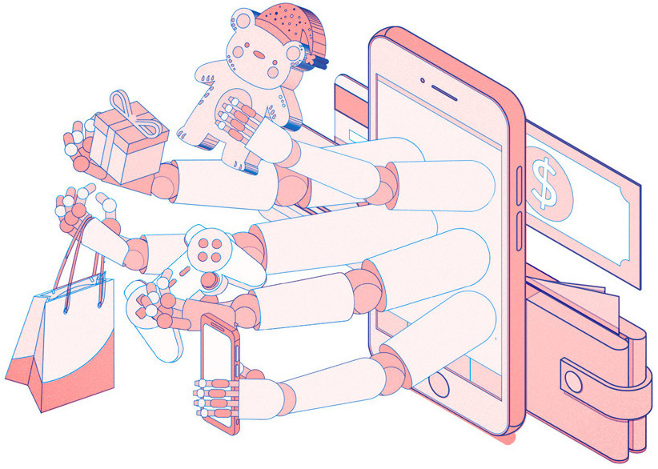
\includegraphics[scale=0.55]{celureco.png}
  \caption{Рекомендатор в ваших руках}
  \label{image:2}
\end{figure}
\newpage

\subsection{Необходимо указать на городские анклавы} Системы рекомендаций используются в электронной торговле, и им удалось монополизировать информацию: на сайте продаж есть вся информация о продуктах, содержании корзины, сделанных покупках и квалификации, которая будет служить для выработки рекомендаций. В обычном магазине это невозможно сделать, и это уменьшает объем продаж того же самого.

В этом новом мире, в котором нормальные магазины стремятся исчезнуть, отрасль стремится разработать все более совершенные алгоритмы для составления рекомендаций, чтобы максимизировать продажи в онлайн-сайтах.

Мы начнем определять систему рекомендаций прототипов, которая использует инструменты этой технологии, но с интересом к определенным группам пользователей, например, к пользователям, которые живут в определенном регионе или районе.

Эта «регионализация», в которой работает наша рекомендательная система, может занять каждый регион как «семью», где жители могут иметь одинаковые вкусы и потребности. В этой модели существуют области более развиты, то есть большее количество развлекательных и культурных мероприятий, мероприятий, которые полезны для улучшения внешнего вида окружающей среды (живопись, садоводство и т.д.), которые требуют продуктов, которые будут куплены или другие услуги типа " доля-экономика "\cite{shared_economy}.

Эти рекомендации могут также использоваться пользователями городских анклавов в целях их развития, принимая их в качестве примера, чтобы эволюционировать их окрестности. Но подумайте, можно ли свергнуть крупные интернет-сайты продаж? Ответ сегодня кажется нет, но правительства начинают обвинять монополистов в крупных сайтах онлайн-продаж, таких как Amazon. Возможно, что в какой-то момент они юридически ограничены для работы в глобальном масштабе или с большими налогами.

Электронная коммерция и запрограммированное устаревание \cite{planned_obsolescence} продуктов, заставляют потребителя повторять покупки, и именно там действуют традиционные системы рекомендаций. Желание покупать товары все быстрее и быстрее не делает людей счастливее.

Хотя невозможно предсказать будущее, если можно подготовиться к более совместной экономике, где рекомендуются не только продукты, но и общий опыт для развития. Система рекомендаций в совместной экономике могла бы:



\begin{enumerate}
\item Предлагайте экономическую экономию, позволяя узнать о интересах пользователей соседства и сотрудничать с предложениями о покупке групп.
\item Большее предложение для потребителя. Лучший доступ к другим альтернативам, которые до сих пор не были жизнеспособными или не были видны большинству из нас.
\item Устойчивое развитие. Совместная экономика поощряет и провоцирует второе использование продуктов.
\item Благоприятные эффекты для соревнований. Это способствует предпринимательству, стимулирует конкуренцию и экономическую активность. Они уже делят квартиры, транспортные средства, транспорт и т.д.
\item Социальная ценность. Содействие социальной сплоченности, солидарности и социальным отношениям, основанным на доверии. Вы можете создавать развлекательные и культурные мероприятия, присутствовать в других районах, но не существующих, в которых вы хотите улучшить.
\item Управление ресурсами. Использование ресурсов является еще одним из основных принципов совместной экономики, поскольку это то, что приносит пользу всем нам. Лучший пример - водитель, который делится своим автомобилем с несколькими пассажирами с близлежащими пунктами назначения.
\item Экологическая выгода. Сокращение производства с меньшими затратами природных ресурсов и меньшим загрязнением.
\end{enumerate}


Традиционные системы сотрудничества не поощряют разработку упомянутых тем, поскольку для них цель состоит в том, чтобы выработать более эффективные рекомендации относительно товаров для покупки.

\subsection{Используемая информация} 
Это применение характеризуется предоставлением рекомендаций пользователям автоматически, на основании уже совершенных действий (покупок, выставленных рейтингов, посещений и т.д.) и приемом от них обратной связи (заказы в магазинах, переход по ссылкам и т.п.).
Рекомендательные системы являются одним из важных разделов интеллектуального анализа данных - Data Mining.

Существует два типа квалификаций: явная и неявная квалификация. Явная квалификация - это те, которые пользователи сознательно и добровольно выразили в отношении предметов: «Мне это нравится», «они не так уж плохи» и «Мне это не нравится», или по рейтингам от 1 до 5, это позже совершить покупку и получить доступ к квалификации. Комментарии также являются плюсом и полезны на выборах.

Неявные оценки получаются при наблюдении за поведением пользователя. То, что пользователь нажимает на элемент, отражает некоторый интерес к нему, особенно если он добавлен в корзину покупок.

Даже принимая конкретный городской анклав, люди, которые ежедневно используют определенные услуги, такие как «собираются обедать или обедать», в какой-то ресторан в этом районе, могут квалифицироваться наиболее «широко»: в зависимости от контекста {обед, ужин} , {для работы, удовольствия}, также квалифицируют выбранное меню {в частности} и в соответствии со вкусом или типом приготовления. Даже частая частота одного и того же пользователя в определенном ресторане и запрос, например, «пицца», можно считать положительным.

В вышеупомянутом случае система рекомендаций в соответствии со всей собранной информацией может составить профиль пользователя, а затем рекомендовать другие близлежащие рестораны в соответствии с интересами, которые уже проявились. 



\subsection{Основные вызовы системы рекомендаций}

\begin{enumerate}
\item
Разнообразие данных. Когда среднее число оценок для каждого пользователя или элемента велико, они могут быть распределены неравномерно, и поэтому есть пользователи или элементы со многими оценками, а другие - с небольшим количеством. В случае предоставления локальных услуг его можно использовать как юниверс для близлежащих пользователей.

\item
Масштабируемость. По мере роста числа пользователей и предметов необходимо учитывать проблемы с вычислительными затратами и искать алгоритмы рекомендации, которые не требуют или не могут быть параллельными (или и теми и теми). Другим возможным решением является использование инкрементных версий алгоритмов, где, по мере роста информации, рекомендации не пересчитываются глобально, а постепенно.

\item
Холодный старт. Когда новый пользователь входит в систему, недостаточно информации для получения рекомендации для него. Хорошая система рекомендаций должна быть в состоянии справиться с этой ситуацией. Вот почему мы подчеркиваем, что, возможно, пользователи одного и того же региона могут иметь аналогичные предпочтения, которые помогают минимизировать холодный старт.

\item
Разнообразие по сравнению с точностью. Когда задача сосредоточена на рекомендации пунктов, которые могут быть оценены конкретным пользователем, обычно более эффективно рекомендовать элементы с высокими и популярными рейтингами. Хороший список рекомендуемых элементов также должен содержать менее очевидные элементы, которые пользователю сложнее выполнить самостоятельно.

\item
Уязвимость к атакам. Учитывая его важность в приложениях электронной коммерции, системы рекомендаций являются объектами атак для продвижения или подавления определенных предметов (этого было бы достаточно, чтобы создать ложные профили пользователей, с тем чтобы сделать положительную квалификацию для тех предметов, которые они хотели бы продвигать, и негативы для тех, кто хотел бы подавить ). Существует широкий набор инструментов, позволяющих избежать этих атак.

\item
начение времени. Есть предметы, которые интересуются только в течение определенного периода времени. Интересно знать, когда следует отклонять старые мнения и каковы временные шаблоны в оценках пользователей и актуальности предметов.

\item
Оценка рекомендаций. У нас есть разные показатели, но выбор лучшего для данной ситуации остается открытым. Сравнение между различными алгоритмами рекомендаций проблематично, потому что они решают разные задачи.

\item
Пользовательский интерфейс. Рекомендации должны быть прозрачными, чтобы пользователь знал, почему эти элементы были рекомендованы. Пользователю должен быть показан длинный список, но он представлен простым способом, и его легко ориентировать. В настоящее время интерфейс имеет очень большое значение, но считается, что в скором времени у нас будет мир без экранов \cite{screenless}, что приведет к усиленной реальности.

\item
Представьте себе, что в будущем системы рекомендаций будут основой стандарта для совершения покупок, но уже не с прокруткой списка пользователей, но одни и те же алгоритмы рекомендуют и совершают покупку. Например, холодильник может контролировать уровни существования пищи и делать заказы на покупку, когда они опускаются ниже определенного порога, выбирая, где покупать в соответствии с системой рекомендаций и совершая платеж через виртуальный кошелек.
\end{enumerate}


\subsection{Cтруктура}

Структура системы рекомендаций имеет форму двудольного графика, в котором на одном из подграфов представлены пользователи, а в других - элементы. Таким образом, дуги графа, которые соединяют пользователей с элементами, представляют собой квалификации между ними.


\begin{figure}[h]
  \centering
  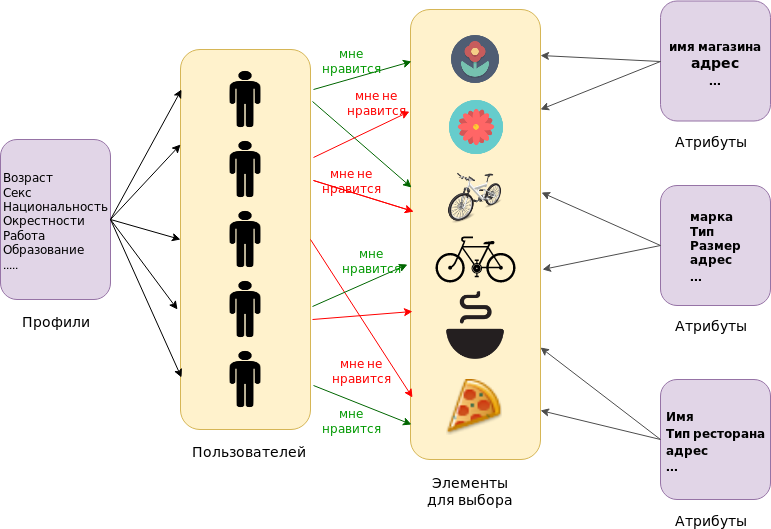
\includegraphics[scale=0.55]{struct_recomm.png}
  \caption{Структура системы рекомендаций}
  \label{image:scheme4}
\end{figure}

Проблема рекомендации может быть определена о том, как дать рекомендации пользователю о новых элементах на основе исторической информации, хранящейся в системе, и предложить этому пользователю новые и оригинальные элементы, для которых предсказанный ответ высок.

Тип ответов пользовательского элемента варьируется от одного приложения к другому и попадает в одну из этих четырех категорий: скалярный (1..5), текстовый (мне нравится, мне нравится, мне это не нравится, не согласен и т. д.), двоичный (мне нравится или мне это не нравится) и, наконец, унарный ответ, который захватывает взаимодействие пользователя с элементом (например, покупка, доступ в Интернет и т. д.) без предоставления явной информации об оценке пользователя для этого элемента.

Поскольку большинство пользователей склонны взаимодействовать с элементами, которые они находят интересными, унарные ответы по-прежнему предоставляют полезную информацию о предпочтениях пользователей.

«Сегодня люди любят оценивать и добавлять рекомендации, но возможно, что в ближайшем будущем унарный ответ может быть единственным признаком.»










\subsection{Формальное определение проблемы: Постановка задачи}
Каждая проблема имеет свою собственную математическую формулировку, поэтому для того, чтобы понять, что мы искали в нашей проблеме, мы описываем ее математическую формулировку.

Прежде всего, набор пользователей, использующих нашу систему, будет обозначаться буквой $U$, а набор элементов - $I$.

Более того, обозначим через R набор рейтингов, записанных в системе, и напишем S набор возможных значений для рейтинга, в этом случае мы будем использовать $S = [1, 5]$. 

Кроме того, мы предполагаем, что любой пользователь u ∈ U для любого элемента $i ∈ I$ может быть не более одного рейтинга и написать $r_{ui}$ этот рейтинг. Чтобы определить подмножество пользователей, которые оценили элемент i, мы используем обозначение $U_{i}$. Аналогично, $I_{u}$ представляет подмножество элементов, которые были оценены пользователем $u$. Наконец, элементы, которые были оценены двумя пользователями $u$ и $v$, то есть $I_{u} \cap I_{v}$, являются важной концепцией в нашей презентации, и мы используем Iuv для обозначения этого понятия. Аналогичным образом, $U{i,j}$  используется для обозначения набора пользователей, которые оценили оба пункта $i$ и $j$.

Двумя наиболее важными проблемами, связанными с системами рекомендаций, являются проблемы с рекомендациями «лучший элемент» и «верхний N». Первая проблема заключается в нахождении для конкретного пользователя u нового элемента $i ∈ I \ I_{u}$, для которого, скорее всего, будет интересен u. Когда рейтинги доступны, эта задача чаще всего определяется как регрессия или ( многоклассовая), задача которой состоит в том, чтобы изучить функцию $f: U \times I \rightarrow  S$, которая предсказывает рейтинг $f\left ( u,i \right )$ пользователя u для нового элемента $i$. Затем эта функция используется, чтобы рекомендовать активному пользователю ua элемент $i^{*}$, для которого оценочная оценка имеет наибольшее значение:

\begin{equation}
i^{*}=\argmax_{j\in I\setminus I_{u}}\\f\left ( u_{a},j \right ).
\label{F:F1}
\end{equation}


\subsection{Метрики оценки}

Точность обычно используется для оценки эффективности метода рекомендации. Как правило, оценки R делятся на обучающий набор Rtrain, используемый для изучения f, и тестовый набор Rtest, используемый для оценки точности прогнозирования. Двумя популярными мерами точности являются средняя абсолютная ошибка $(MAE)$:

\begin{equation}
MAE (f)=\frac{1}{|R_{test}|}\sum_{r_{ui}\in R_{test}}^{n}|f(u,i)-r_{ui})| \\.
\label{F:F2}
\end{equation}

и Root Mean Squared Error $(RMSE)$:


\begin{equation}
RMAE (f)=\sqrt{\frac{1}{|R_{test}|}\sum_{r_{ui}\in R_{test}}^{n} \left ( f(u,i)-r_{ui} \right )^{2} }\\.
\label{F:F3}
\end{equation}


Если рейтинги недоступны, например, если известен только список предметов, приобретенных каждым пользователем, измерение точности прогноза рейтинга невозможно. В таких случаях проблема поиска лучшего предмета обычно превращается в задачу рекомендовать активному пользователю ua список L (ua), содержащий N элементов, которые могут его заинтересовать \cite{topn}. Качество такого метода можно оценить, разбив элементы I на набор $I_{train}$ , используемый для изучения $L$, и тестовый набор $I_{test}$. Пусть $T\left ( u \right )\subset I_{u}\cap I_{test}$ - подмножество тестовых элементов, которые пользователь u нашел релевантным. Если ответы пользователя являются бинарными, это могут быть элементы, которые u положительно оценили. В противном случае, если для каждого пользователя u предоставляется только список приобретенных или доступных элементов, то эти элементы могут использоваться как $T\left ( u \right )$. Выполнение метода затем вычисляется с использованием мер точности и отзыва:

Точность - это соотношение между количеством полученных документов и количеством полученных документов. Таким образом, чем ближе значение точности приближается к нулевому значению, тем больше количество восстановленных документов, которые они не считают релевантными. Если, напротив, значение точности равно единице, то будет понятно, что все восстановленные документы имеют значение.
\\
\begin{equation}
Precision =\frac{1}{\left | U \right |}*\sum_{u\in U}^{  } \left |L\left ( U \right )\cap  T\left ( U \right ) \right |/\left | L\left ( U \right ) \right |\\.
\label{F:F4}
\end{equation}

Отзыв- Это соотношение отражает долю соответствующих документов, восстановленных, по сравнению с общим количеством документов, которые имеют отношение к базе данных, независимо от того, были ли они восстановлены или нет.
\begin{equation}
Recall =\frac{1}{\left | U \right |}*\sum_{u\in U}^{  } \left |L\left ( U \right )\cap  T\left ( U \right ) \right |/\left | T\left ( U \right ) \right |\\.
\label{F:F5}
\end{equation}



\begin{figure}[h]
  \centering
  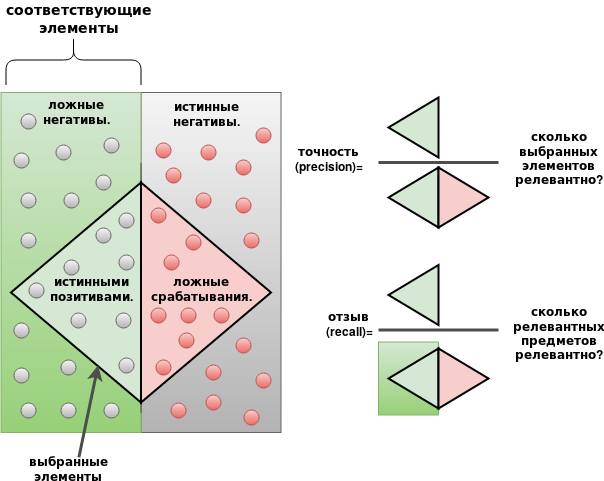
\includegraphics[scale=0.55]{recall.png}
  \caption{Точность и отзыв.}
  \label{image:scheme7}
\end{figure}



Недостатком этой задачи является то, что все элементы списка рекомендаций $L\left ( u \right )$ считаются одинаково интересными для пользователя $u$. Альтернативная настройка, описанная в \cite{topn}, состоит в изучении функции $L$, которая отображает каждого пользователя $u$ в список $L\left ( u \right )$, где элементы упорядочены по своей «интересности» на $u$. Если тестовый набор создается случайным образом, для каждого пользователя u, одного элемента iu Iu, производительность $L$ может быть оценена с помощью Среднего Взаимного $Хит-Ранга (ARHR)$:


\begin{equation}
ARHR(L)=\frac{1}{\left | U \right |}*\sum_{u\in U}^{  } \frac{1}{rank(i_{u},L(u))}\\.
\label{F:F6}
\end{equation}

где $rank \left ( I_{u},L\left (u  \right ) \right )$ - ранг элемента $RHR(L)$ $I_{u}$ в $L\left (u  \right )$, равный $\infty$, если $I_{u}\notin  L_{u}$.
\textit{«Вот строятся математические формулы»}\\



Прежде чем приступать к изучению алгоритмов, мы изучим набор метрики \cite{topn}. Как правило, набор квалификаций делится на два подмножества: «ET» - это подмножество квалификаций, которые будут использоваться в качестве учебного набора, то есть для составления прогнозов; С другой стороны, «EP» будет подмножеством, которое будет сравниваться с соответствующими прогнозами для оценки эффективности рекомендаций.




\newpage
\section{Архитектура и подходы рекомендательная системы}

\begin{figure}[h]
  \centering
  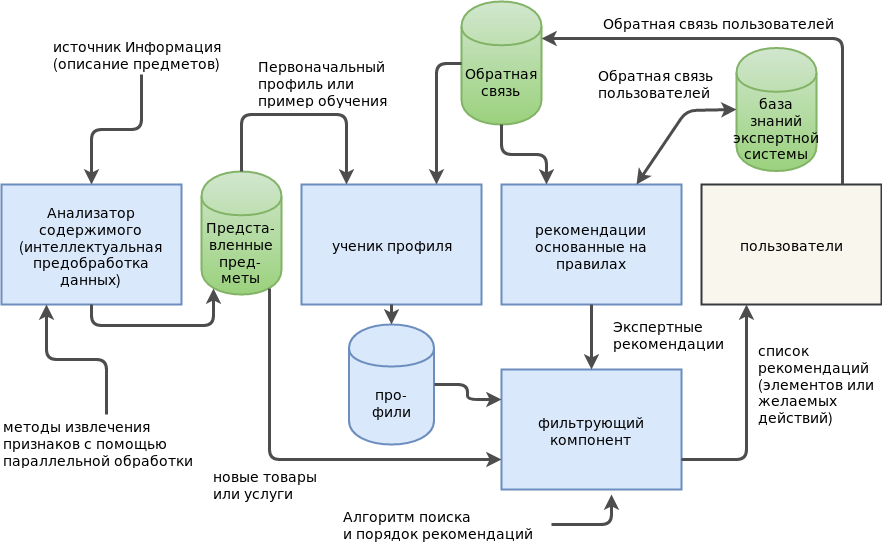
\includegraphics[scale=0.55]{struct_sys.png}
  \caption{ССхема, выбранная для выбранной рекомендательная системы}
  \label{image:scheme6}
\end{figure}

\subsection{Архитектура}
Архитектура системы предусматривает несколько экземпляров, которые обмениваются информацией, в основном отзывами пользователей и ссылкой на предложения продуктов и услуг. Самое подходящее, что каждый город или район могут управлять своей информацией. Данные пользователя являются частью конфиденциальной информации, которая не является общей.

\subsection{Обратная связь}
Обратная связь - это самая важная информация об этой архитектуре, выбор пользователя служит не только для совместной работы с алгоритмами для разработки рекомендаций, но также дает информацию об использовании и обычаях каждого региона. В свою очередь, эта информация служит для сравнения окрестностей с точки зрения разных вариантов по каждой теме и для предоставления наилучших предложений.

\subsection{Передача данных между экземплярами}
Для обмена информацией между экземплярами рассматриваются две альтернативы, первая заключается в том, что каждая система рекомендаций является частью «архитектуры HLA высокого уровня» \cite{hla}, которая делится данными и синхронизирует информацию с другими системами через «Runtime инфраструктуры RTI» \cite{rti} и действовать в симуляции. Вторая - архитектурно-ориентированная сервис-ориентированная архитектура (SOA), где обмен информацией распределяется между службами в архитектуре с низким уровнем связи, используя веб-службы RESTFul. Из-за сложности присущего слоя первого варианта выбирается архитектура API Rest.

\subsection{Защита данных и уведомление}
Информация в данных профиля локальна и не используется. Эти данные принадлежат пользователям, которые живут по соседству. Система предупреждений и уведомлений для пользователей о новых продуктах и мероприятиях или просто рекомендации предупреждает о событиях. Сама система может считаться сервисом или набором услуг.

\subsection{Свободное и открытое программное обеспечение}
Набор функциональных возможностей формирует группу (анализатор данных, менеджер профилей, фильтрацию) и данные: профили пользователей, отзывы и совместную поддержку (данные, планы и правила). Первое не разделяется, а два других.

\newpage
\subsection{Подходы «Content-Based»}
"Content-based" фильтрация предоставляет альтернативные элементы, которые контекстуализируются для просматриваемого элемента.

Система сопоставляет атрибуты элемента, просмотренного с атрибутами других элементов, для генерации рекомендаций, чтобы найти те атрибуты, которые относятся к определенному продукту.

Этот подход основан на описаниях пользовательских предпочтений и предметов, которые они просмотрели или приобрели в прошлом.


\begin{enumerate}
\item «Content-based» Фильтрация  предоставляет альтернативные элементы, которые контекстуализируются для просматриваемого элемента.
\item Система сопоставляет атрибуты элемента, просмотренного с атрибутами других элементов, для генерации рекомендаций, чтобы найти те атрибуты, которые относятся к определенному продукту.
\end{enumerate}

\begin{figure}[h]
  \centering
  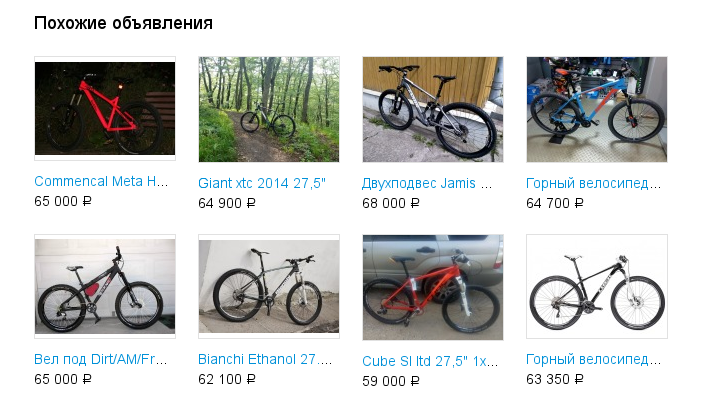
\includegraphics[scale=0.55]{bicis.png}
  \caption{Аналогичные элементы, как выбор пользователя}
  \label{image:scheme5}
\end{figure}


\subsection{TD/IDF}
Чтобы найти эти атрибуты, более релевантные для определенного элемента, мы используем методы «NLP», такие как «TF/IDF».

Модель векторного пространства на основе ключевых слов
Наиболее "content-based" систем рекомендаций на основе контента используют относительно простые модели поиска, такие как сопоставление ключевых слов или модель векторного пространства (VSM) с базовым взвешиванием TF-IDF. VSM представляет собой пространственное представление текстовых документов. В этой модели каждый документ представлен вектором в n-мерном пространстве, где каждый размер соответствует термину из общей лексики данного набора документов.

Формально каждый документ представляется в виде вектора весовых коэффициентов, где каждый вес указывает степень ассоциации между документом и термином. Пусть $D=  d_{1},d_{2},...,d_{n}$ обозначает набор документов или corpus, а $T=  t_{1},t_{2},...,t_{n}$ - словарь, т. Е. набор слов в корпусе. T получается путем применения некоторых стандартных операций обработки естественного языка, таких как токенизация, удаление стоп-слов и создание. Каждый документ d j представлен как вектор в n-мерном векторном пространстве, поэтому  $d_{j}=  w_{1,j},w_{2,j},...,d_{n,j} $, где $w_{k,j}$ - вес для члена $t_{k}$ в документе $d_{j}$.

Представление документов в VSM вызывает два вопроса: взвешивание терминов и измерение сходства вектора признаков. Наиболее часто используемая терминологическая Типосхема взвешивания, TF-IDF (временная частота-обратная документальная частота), основана на эмпирических наблюдениях.


\begin{itemize}
    \item редкие термины не менее важны, чем частые термины (предпосылка IDF).
    \item множественные появления термина в документе не менее важны, чем отдельные случаи (предположение TF).
    \item длинные документы не являются предпочтительными для коротких документов (предположение о нормализации).
\end{itemize}


Другими словами, термины, которые часто встречаются в одном документе (TF =term-frequency), но редко в остальной части корпуса (IDF = частота обратного документа), больше вероятно, будут иметь отношение к теме документа. Кроме того, нормализация полученных весовых векторов предотвращает получение более длинных документов с большей вероятностью извлечения. Эти предположения хорошо иллюстрируются функцией TF-IDF:




\begin{equation}
tdidf\left ( t,d,D \right )=tf(t,d)*idf(t,D)\\.
\label{F:F7}
\end{equation}

\begin{equation}
tf(t,d)=0.5+0.5*\frac{f_{t,d}}{max\left \{ f_{t^{'},d}:t^{'}\in d \right \}}\\.
\label{F:F8}
\end{equation}

\begin{equation}
\left. \begin{matrix}
td \;\;  is\; high\\ 
idf\; is \;low
\end{matrix} \right \} \Rightarrow High\: TD/IDF\\.
\label{F:F9}
\end{equation}
\newpage
\subsection{Архитектура «Content-Based» систем}

\begin{figure}[h]
  \centering
  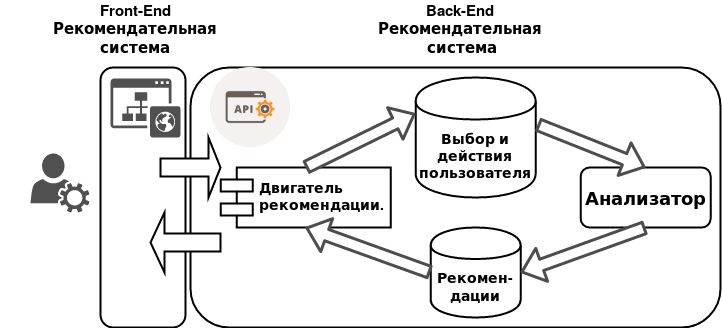
\includegraphics[scale=0.55]{content.png}
  \caption{Структура системы рекомендаций}
  \label{image:scheme8}
\end{figure}
Три отдельных модуля «Анализатор содержимого», «ученик профиля» и «Фильтрующий компонент», которые отвечают за процесс рекомендации, используя надлежащие методы для представления элементов и создания профиля пользователя, а также некоторые стратегии для сравнения профиля пользователя с представлением элемента.

Анализатор содержимого
В базе данных мы можем хранить данные в таблицах, и нетрудно получить информацию, использующую, например, команды SQL, но когда данные не имеют структуры (например, opioions, размещенные на веб-сайтах, веб-страницах, новостях, описаниях продуктов и т. Д.), Поступающих из разных источников в более подходящий источник восстановления через задачи предварительной обработки в другом, чтобы извлечь структурированную релевантную информацию. Это основная задача анализатора контента, но она является высокопоставленным потребителем, технология использует новые технологии для таких задач, как Apache Hadoop или Spark, которые хранят информацию в «озерах данных» \cite{lakes} больше полезной для обработки больших данных, в режиме реального времени аналитика и машинное обучение для лучшего решения.


Элементы данных анализируются с помощью методов извлечения признаков, чтобы переместить представление позиции из исходного информационного пространства в целевое (например, веб-страницы, представленные как векторы ключевых слов).

Первым шагом процесса рекомендации является тот, который выполняется «Анализатором содержимого», который обычно заимствует методы из систем поиска информации \cite{retrieve}. Описание описаний, исходящих из Источника информации, обрабатывается с помощью анализазаторского содержимого, которое извлекает функции (ключевые слова, n-граммы, концепции и т. Д.) Из неструктурированного текста для создания структурированного представления элемента, хранящегося в репозитории «Представленные элементы».

Эта предварительно обработанная информация представляет собой вход для модулей «Изучение профиля» и «фильтрующий компонент».

Модуль «Изучение профиля» собирает данные данных пользователя и использует методы машинного обучения для создания профиля пользователя, чтобы иметь возможность выводить модель интересов пользователей, начиная с предметов, которые нравились или не нравились в прошлом. Также модуль реализует метод обратной связи обратной связи \cite{retrieve}, в котором метод обучения объединяет векторы положительных и отрицательных примеров в векторе прототипа, представляющем профиль пользователя.

\begin{figure}[h]
  \centering
  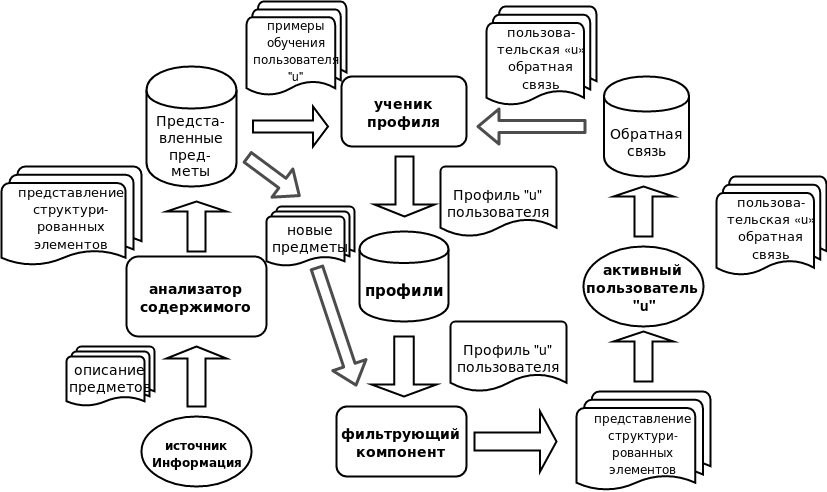
\includegraphics[scale=0.55]{hla.png}
  \caption{Архитектура «Content-Based» систем}
  \label{image:scheme9}
\end{figure}

Модуль «Фильтрующий компонент» использует профиль пользователя, чтобы предлагать соответствующие элементы, сопоставляя представление профиля с параметром, рекомендуемым для элементов. Результатом является суждение, сравнивая предпочтения в представлении элемента с элементами в пользовательских предпочтениях (хранящихся в профиле пользователя). Результат в ранжированном списке потенциально интересных предметов. Согласование выполняется путем вычисления сходства косинусов между вектором прототипа и векторами предметов.

Пользовательские вкусы обычно меняются со временем, поэтому предпочтения должны поддерживаться и предоставляться «Изучение профиля», чтобы автоматически обновлять профиль пользователя. Когда пользователи сообщают о своем удовлетворении или неудовлетворенности выбранными позициями, обратная связь заключается в том, что процесс обучения снова выполняется в новом наборе тренировок, и полученный профиль адаптирован к обновленным интересам пользователей.
\subsection{Создание профиля и отзывов в явных оценках}

Чтобы создать пользовательский профиль, должен быть определен обучающий набор для пользователя. Учебный набор представляет собой пары $⟨i_{k}, r_{k}⟩$, где $r_{k}$ - это рейтинг, предоставляемый ua в представлении элемента I k.

Учитывая набор позиций, помеченных рейтингом, «Изучение профиля» применяет контролируемые алгоритмы обучения для создания предсказательной модели, которая хранится в «репозитории профилей» для последующего использования «фильтрующим компонентом».

Чтобы создать и обновить профиль активного пользователя ua (пользователя, для которого должны быть предоставлены рекомендации), ее реакция на элементы собирается каким-то образом и записывается в репозиторий «Обратная связь»\cite{retrieve}.

\subsection{Определение, преимущества и недостатки}
\subsection{Алгоритмы «Content-Based»}

\subsection{Построение «Рекомендательная система»}
\subsection{Анализ требований}
\subsection{Анализ и разработка решения}


\subsection{Подходы «Коллаборативная фильтрация»}


Совместная фильтрация - это метод автоматического прогнозирования (фильтрации) об интересах пользователя путем сбора предпочтений или информации о вкусе у других пользователей (сотрудничающих).


Он предполагает, что если у человека А есть такое же мнение, как у человека в вопросе, у А более вероятно, что мнение Б будет по другому вопросу, чем у случайно выбранного человека.

\begin{figure}[h]
  \centering
  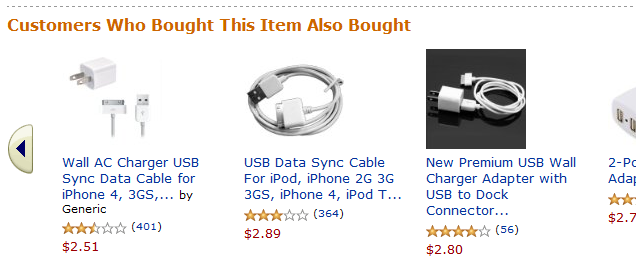
\includegraphics[scale=0.65]{others.png}
  \caption{Предложения от другого выбора пользователя}
  \label{image:scheme10}
\end{figure}

Типы: Пользователь к пункту: лучшее преобразование, но сложнее вычислить
Элемент к пункту: меньше времени зависит, но менее эффективно.

Альтернативные наименьшие квадраты или ALS являются более распространенным алгоритмом CF и являются методом матричной факторизации.
Он разлагает матрицу оценок пользовательских позиций на две части:


\begin{itemize}
    \item Пользовательская матрица с ней скрытые факторы (характеристики).
    \item Транспонирование матрицы элементов со своим скрытым фактором.
\end{itemize}

\begin{figure}[h]
  \centering
  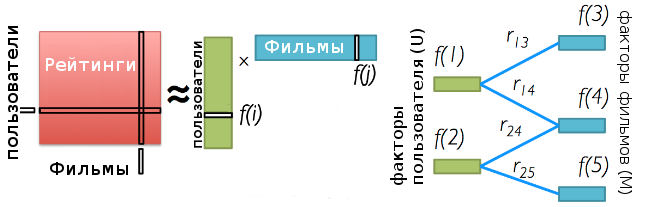
\includegraphics[scale=0.7]{descompo.png}
  \caption{Разделить рейтинги «пользовательский элемент»}
  \label{image:scheme11}
\end{figure}

В основном существуют два типа систем рекомендаций: «на основе контента» и «совместная фильтрация». В системах рекомендаций «на основе контента» система учитывает только квалификацию (неявную или явную), которую пользователь, получивший рекомендацию, сделал на некоторых элементах заранее. На основе этих квалификаций прогнозируется рейтинг, который пользователь предоставит остальным элементам, составляющим систему, и пользователю с наивысшим прогнозируемым значением предлагается пользователю.

Системы рекомендации типа «Коллаборативная фильтрация» наиболее часто используются в наши дни, поскольку с учетом квалификации всех пользователей системы могут предлагаться более разнообразные рекомендации, но с учетом оценки пользователя.

Основная идея заключается в том, что рейтинг «$u$» для нового элемента «$i$», скорее всего, будет похож на рейтинг другого пользователя «$v$», если «$u$» и «$v$» оценили другие элементы аналогичным образом. Аналогичным образом, «u», вероятно, будет оценивать два элемента «$i$» и «$j$» аналогичным образом, если другие пользователи дали аналогичные рейтинги этим двум элементам.

Начнем с примера: «Amazon» \cite{amazon} использует систему рекомендаций для совместной фильтрации, чтобы предлагать рекомендации своим пользователям. Первоначально, когда пользователь является новым, он предлагает рекомендацию «по отдельности», предлагающую рекомендации, основанные на элементе, который пользователь недавно видел. То есть, если пользователь посетил ссылку в «ремонте дома», связанную с «Живописью для белых фасадов», следующая вещь, которую система порекомендует, будет другими типами «покрытие для фасадов домов» или «краска для внешней», ». Таким образом, это позволяет избежать холодного начала, с которым страдают системы рекомендаций, когда у них мало информации.

Позже, когда система получает больше информации о пользователе (он проявляет интерес к большему количеству продуктов или предметов) и может избежать холодного запуска, он уже использует систему рекомендаций «пользователь для пользователя», то есть он ищет пользователя текущие среди остальных наиболее похожих, те, кто видел или купил те же предметы. Из интересов этих пользователей предлагаются рекомендации к текущему.

Он также использует глобальные алгоритмы факторизации, то есть сравнивает несколько характеристик для каждого элемента и присваивает им вес, чтобы впоследствии иметь возможность вычислять сходство между элементами с учетом нескольких факторов и определять приоритеты тех, для которых пользователь проявляет больше интереса.

Ниже приведены два алгоритма совместной фильтрации с различными способами получения прогнозов:

\subsection{Определение, преимущества и недостатки}

Сильные стороны, которые выделяются в алгоритме, делают это как с начала операции, в то время как система растет экспоненциально, надежность, эффективность и стоимость работы поддерживаются.

Простота: этот метод относительно прост для реализации и интуитивно понятен, и только количество соседей, используемых в предсказании, должно быть установлено как параметр. Лучше начать с алгоритма, который мы можем понять.

Обоснованность: дать доверие к результатам обоснование в необходимом. Например, в рекомендации, основанной на элементах, список соседних элементов, а также рейтинги, предоставленные пользователем этим элементам, могут быть представлены пользователю в качестве обоснования для рекомендации. Кроме того, пользователи по соседству могут понять значимость рекомендаций, а также служить основой для интерактивной системы, в которой пользователи могут выбирать соседей, для которых большее значение должно быть дано в рекомендации.

Эффективность. Одной из сильных сторон систем, основанных на окрестности, является их эффективность. В отличие от подхода, основанного на модели, он не требует дорогостоящих этапов обучения, а ближайших соседей можно предварительно вычислить в автономном режиме, обеспечивая почти мгновенные рекомендации. Более того, хранение этих ближайших соседей требует очень небольшой памяти, что делает такие подходы масштабируемыми для приложений, имеющих миллионы пользователей и элементов. Нет необходимости иметь большую инфраструктуру.

Стабильность: Еще одно полезное свойство этого подхода заключается в том, что новые пользователи, элементы и рейтинги могут быть добавлены, а система будет стабильной, не нужно тренироваться снова и когда новые оценки будут введены для нового элемента, только сходство между этим элементом и которые уже в системе должны быть вычислены.


\subsection{Алгоритмы «Коллаборативная фильтрация»: Алгоритм соседнего K}


Алгоритм соседнего K является одним из наиболее употребительных в библиографии, так как это очень простой алгоритм с достаточно точными результатами. Проблема возникает, когда вы намерены использовать ее в очень большой системе, поскольку масштабируемость не является одним из ее преимуществ: за счет увеличения объема данных количество операций, необходимых для рекомендации, значительно увеличивается. Существуют две версии этого алгоритма: алгоритм соседнего пользователя «пользователь к пользователя» и алгоритм соседнего элемента K «элемент к элементу»; в обоих случаях фиксированное число соседей может быть заменено порогом подобия, чтобы выбирать только соседей, которые достигают определенного уровня подобия.

Алгоритм соседнего пользователя K "пользователю"
Эта версия алгоритма основана на идее, что аналогичные пользователи будут одинаково квалифицировать один и тот же элемент. Он состоит из трех этапов:



\begin{enumerate}
	\item Используя выбранную меру подобия, строится набор соседнего K целевого пользователя $a$. Соседние $K$ будут теми, для которых большее сходство получается с пользователем $a$.
	\item Как только пользователи $K$, наиболее близкие $к$ пользователю (соседи), уже получены, чтобы вычислить предсказание этого пользователя для элемента $i$, функция агрегации применяется $к$ рейтингам, которые соседние $K$ сделали на пункт $i$.
	\item Чтобы получить $n$ лучших рекомендаций, мы выбираем $n$ элементов, которые обеспечивают пользователю большее удовлетворение в соответствии с прогнозами.
\end{enumerate}


Этот подход обеспечивает хорошие результаты с достаточно заполненной БД, но когда пользователь не выдал много рейтингов, трудно найти достаточно похожих соседей, и происходит так называемый холодный старт.

Он также должен иметь дело с проблемой вышеупомянутой масштабируемости, поскольку для того, чтобы предлагать рекомендации для пользователя, его подобие с каждым из пользователей системы должно быть рассчитано, что-то с очень высокой вычислительной стоимостью.

Алгоритм соседнего элемента $K$ "элемент $к$ элементу"
Версия «по отдельности» алгоритма значительно снижает проблему малой масштабируемости. В этом случае соседи вычисляются для каждого элемента и сохраняются для использования при расчете прогнозов. Эта информация устарела, но она менее чувствительна к хранению неточной информации об элементах, чем о пользователях.


Этапы этого подхода:
\begin{enumerate}
	\item Определите q соседних элементов каждого элемента системы.
	\item Для каждого элемента $i$, не оцененного целевым пользователем a, вычислить прогноз, основанный на оценки, которые он сделал в отношении соседей $i$.
	\item Выберите $n$ лучших рекомендаций для пользователя a из прогнозов шага выше.
\end{enumerate}



%\section{Основы краудсорсинга для совместной экономики}

\textbf{Разъём TRS} (аббревиатура от англ. Tip, Ring, Sleeve — кончик, кольцо, гильза; подразумевается форма контактов на штекере) — распространённый разъём для передачи аудиосигнала. \cite{wiki-trs}

Однако, наверное мало кто из тех, кто сталкивался с этими разъемами в быту слышал, что они называются TRS, а все потому что у нас прижилось другое название. Его часто называют просто <<джек>>, и это никак не связано с какой-нибудь личностью по имени Джек: на самом деле с английского языка слово <<jack>> переводится как <<гнездо>>. Причем джеком правильно называть именно гнездо, то есть куда подключается, а это разъём-мама на панели, то есть на системном блоке или другом устройстве, а разъем-папу называют plug, что и переводится как <<штекер>>. \cite{kkg-jack}

\textbf{Джек (jack)} - это разъем диаметром 1/4 дюйма (6,3 мм). Применяется в музыкальном оборудовании, чаще всего Вы с ними встретитесь при использовании:
\begin{enumerate}
\item микрофонов для любителей (чаще всего это караоке или для домашней записи)
\item электрогитар, бас-гитар, педалей (<<примочек>>), усилителей для гитары.
\item профессиональных наушников
\item профессиональных звуковых плат
\end{enumerate}

\textbf{Мини-джек (mini-jack)} - разъём диаметром 3,5 мм. По сравнению с джеком действительно <<мини>>, и используется в устройствах, где размер действительно важен. Его вы можете встретить, купив:
\begin{enumerate}
\item наушники (обычные наушники для плеера, к примеру)
\item компьютерную акустичекую систему (её называют динамики или же колонки) 
\item гарнитуру
\item плеер
\item звуковую плату потребительского уровня
\end{enumerate}

\begin{figure}[h]
  \centering
  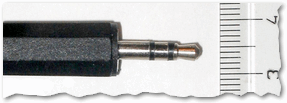
\includegraphics[scale=1]{mini-jack-audio.png}
  \caption{Разъем мини-jack}
  \label{image:mini-jack-audio}
\end{figure}

\begin{figure}[h]
  \centering
  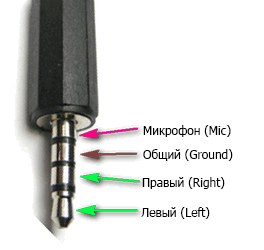
\includegraphics[scale=1]{headset.png}
  \caption{Гарнитурный штекер}
  \label{image:headset}
\end{figure}

На ноутбуках есть два вида разъемов, предназначеных для подключения акустической системы и микрофона. Они показаны на Рисунке ~\ref{image:notebook}. Для подключения гарнитуры с стандартным совмещенным штекером (Рисунок ~\ref{image:headset}) в левый разъем (Рисунок ~\ref{image:notebook}) используется переходник, показанный на рисунке ~\ref{image:adapter}.

\begin{figure}[h]
  \centering
  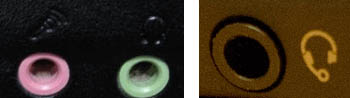
\includegraphics[scale=1]{notebook.jpg}
  \caption{Разъемы ноутбука}
  \label{image:notebook}
\end{figure}

\begin{figure}[h]
  \centering
  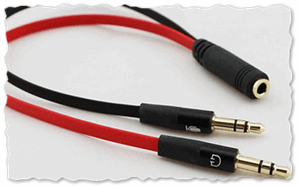
\includegraphics[scale=1]{adapter.png}
  \caption{Переходник для подключения гарнитурных наушников к обычной звуковой карте}
  \label{image:adapter}
\end{figure}

\section{Звуковая архитектура}

Рисунок \ref{image:sound_arch} показывает подключение звука на ПК-совместимой системе. Аудио контроллер Южного моста, а также внешний кодек, подключённый к аналоговой звуковой схеме. \cite{eldd}

\begin{figure}[h]
  \centering
  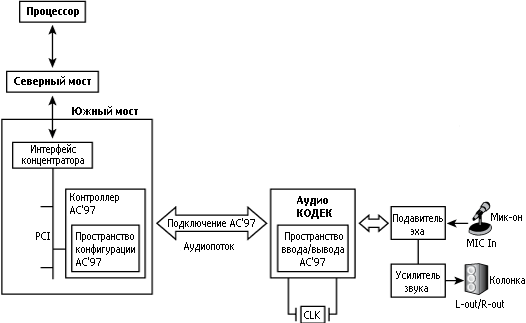
\includegraphics[scale=0.8]{sound_arch.png}
  \caption{Звук в среде ПК}
  \label{image:sound_arch}
\end{figure}

\subsection{Звуковая подсистема Linux}

\subsection{Open Sound System}
\textbf{Open Sound System} (OSS) — унифицированный драйвер для звуковых карт и других звуковых устройств в различных UNIX-подобных операционных системах.

OSS основан на Linux Sound Driver и в настоящее время работает на большом числе платформ: Linux, FreeBSD, OpenSolaris и т. д. \cite{wiki-oss}

/dev/dsp и /dev/audio — основные файлы устройств для цифровых приложений. Любые данные, записанные в эти файлы, воспроизводятся на DAC/PCM/DSP устройстве звуковой карты. Чтение из этих файлов возвращает звуковые данные, записанные с текущего входного источника (по умолчанию это Микрофонный вход).

При чтении из /dev/dsp мы получаем несжатый аудиопоток с микрофона компьютера через вход звуковой карты. 

\subsection{ALSA}

\textbf{ALSA} (англ. Advanced Linux Sound Architecture, Продвинутая звуковая архитектура Linux) — архитектура звуковых драйверов, а также широкий их набор для операционной системы Linux, призванный сменить Open Sound System (OSS). ALSA тесно связана с ядром Linux. ALSA — программный микшер, который эмулирует совместимость для других слоев. Также предоставляет API для программистов и работает с низкой стабильной задержкой. \cite{wiki-alsa}

ALSA является звуковой подсистемой, выбранной  для ядра версии 2.6. Открытая Звуковая Система, OSS, звуковой уровень в ядре версии 2.4, в настоящее время устарел и не рекомендуется к использованию. Для перехода от OSS к ALSA последняя предоставляет эмуляцию OSS, которая позволяет приложениям, использующим API OSS, запускаться без изменений на ALSA. Звуковые ядра Linux, такие как ALSA и OSS, делают аудио приложения независимыми от базового оборудования.

Чтобы понять архитектуру звуковой подсистемы Linux посмотрите на Рисунок  \ref{image:sound_system}. 

\begin{figure}[h]
  \centering
  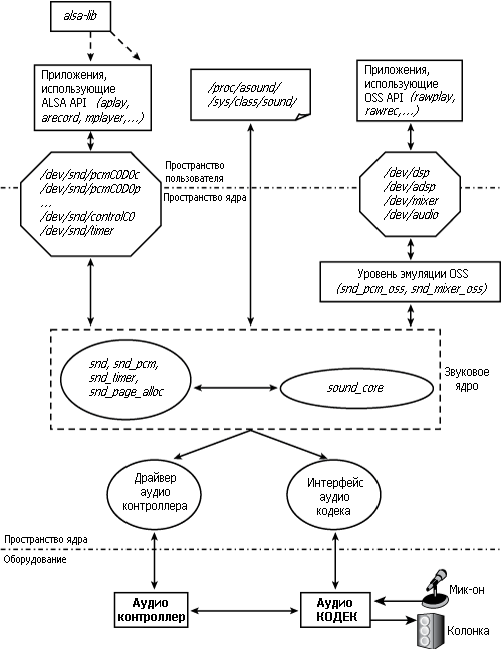
\includegraphics[scale=0.8]{sound_system.png}
  \caption{Звуковая подсистема Linux (ALSA)}
  \label{image:sound_system}
\end{figure}

Основными частями подсистемы являются:

\begin{enumerate}
\item Звуковое ядро, которое является базовым кодом, состоящим из процедур и структур, доступных другим компонентам звукового уровня Linux. Как и уровни ядра, принадлежащие другим драйверным подсистемам, звуковое ядро обеспечивает уровень косвенности, что делает каждый компонент в звуковой подсистеме не зависящим от других. Ядро играет важную роль в экспорте API ALSA вышележащим приложениям. Узлами /dev/snd/*, показанными на Рисунке \ref{image:sound_system}, которые создаются и управляются из ядром ALSA, являются: /dev/snd/controlC0 - узел управления (используемый в приложениях для управления уровнем громкости и тому подобному), /dev/snd/pcmC0D0p - устройство воспроизведения (p в конце имени устройства означает playback, воспроизведение), и /dev/snd/pcmC0D0c - записывающее устройство (c в конце имени устройства означает capture, захват). В этих именах устройств целое число после C является номером карты, а после D - номером устройства. ALSA драйвер для карты, которая имеет голосовой кодек для телефонии и стерео кодек для музыки, может экспортировать /dev/snd/pcmC0D0p для чтения аудио потоков, предназначенный для первого, и /dev/snd/pcmC0D1p для качественного музыкального канала для последнего.
 
\item Драйверы аудио контроллера зависят от оборудования контроллера. Например, для управления аудио контроллером, находящимся в Южном мосте Intel ICH, используется драйвер snd\_intel8x0.
 
\item Интерфейсы аудиокодеков, которые помогают взаимодействию между контроллерами и кодеками. Для кодеков AC'97 используйте snd\_ac97\_codec и модули ac97\_bus.
 
\item Уровень эмуляции OSS, который выступает в качестве посредника между приложениями, использующими OSS, и ядром с поддерживающим ALSA. Этот уровень экспортирует узлы /dev, изображающие поддержку уровня OSS в ядре версии 2.4. Эти узлы, такие как /dev/dsp, /dev/adsp и /dev/mixer, позволяют приложениям OSS работать поверх ALSA без изменений. Узел OSS /dev/dsp связан с узлами ALSA /dev/snd/pcmC0D0*, /dev/adsp соответствует /dev/snd/pcmC0D1*, а /dev/mixer связан с /dev/snd/controlC0.
 
\item Интерфейс procfs and sysfs для доступа к информации через /proc/asound/ и /sys/class/sound/.
 
\item Библиотека ALSA пользовательского пространства, alsa-lib, которая предоставляет объект libasound.so. Эта библиотека упрощает работу программиста приложения ALSA, предлагая несколько готовых процедур для доступа к драйверам ALSA.

\item Пакет alsa-utils, который включает в себя такие утилиты, как alsamixer, amixer, alsactl и aplay. alsamixer или mixer используются для изменения громкости звуковых сигналов, таких как линейный вход, линейный выход или микрофон, а alsactl - для управления параметрами драйверов ALSA. aplay используется для воспроизведения звука через ALSA.
\end{enumerate}

В данной работе для получения потока байтов от микрофонного разъема будем использовать API, предоставляемые ALSA.

\newpage
\section{Управление инцидентами инфраструктуры района или города}

\subsection{Анализ процесса поддержки развития районов}

\begin{figure}[h]
  \centering
  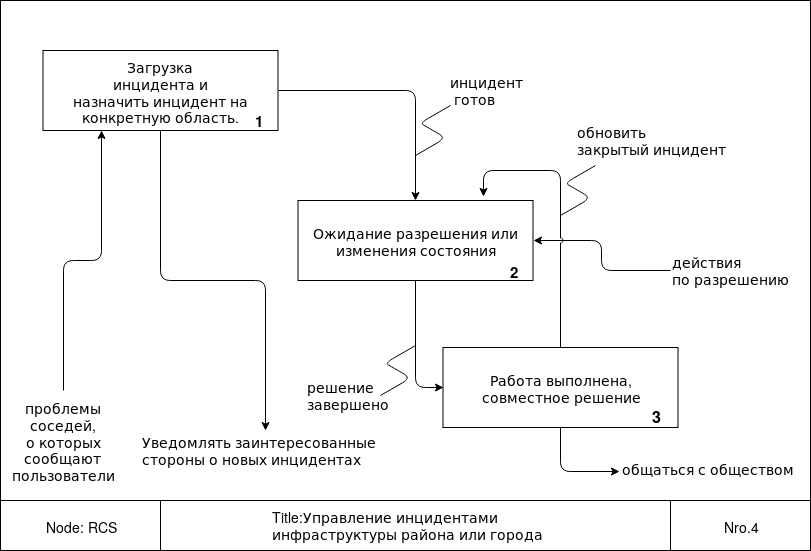
\includegraphics[scale=0.55]{diag_incid.png}
  \caption{Структура системы рекомендаций}
  \label{image:scheme13}
\end{figure}

\begin{table}[]
\centering
\begin{tabular}{|p{4cm}|p{10cm}|}
\hline
\multicolumn{2}{|p{14cm}|}{Область запроса и отдельные подразделы} \\ \hline
Проблемы и улучшения в парках для детей.
& Ремонт.
Увеличения.
Изменения.    \\ \hline
Совершенствование парков и лесов.
& Очистка.
Заказ области.
Безопасность.   \\ \hline
Проблемы в пешеходных зонах.
&  Очистка.
Ремонт тротуаров.
Свет и безопасность.   \\ \hline
Организация дорожного движения.
& Предложения по улучшению трафика.
Заявка на снятие транспортного средства   \\ \hline

\end{tabular}
\centering
\caption{Запрос области.}
\centering
\label{tabla:sencilla3}
\end{table}
\newpage
\section{Усовершенствования для соседства, идеи от пользователей}

\subsection{Районы и Сообщество}

Районы постоянно развиваются, в основном новые, которые формируются, это ясно, так как многое предстоит сделать. Некоторые из них достигли большей эволюции, чем другие. В эволюции соседства происходит несколько факторов, есть экономический фактор, который способствует, а также коллективный дух тех, кто их обитает.

В то время как часть ответственности за улучшения, поддержание и эволюция окрестностей принадлежит государству, другая часть несет ответственность за людей, которые населяют ее. В мире, который работает так быстро, существует нехватка коллективного сознания, необходимого для развития как сообщества.

Другие факторы вмешиваются в эволюцию окрестностей, такие как отсутствие диалога между жителями или незнание целей как общества, но анализ их выходит за рамки этого проекта.

\subsection{Анализ существующей потребности}

Чтобы способствовать эволюции окружающей среды, в которой живет сообщество, необходимо иметь полезную информацию и инструменты, которые позволяют свободно выбирать и использовать доступные альтернативы, различные улучшения как для жилья, так и для окружающей среды.

Принимая в качестве окружения окрестности, в которой живет «гражданин», у него есть профиль предпочтений или предпочтений ссылки по каждому предмету, и он предназначен для прогнозирования «ранжирования» или взвешивания, которые пользователь дал бы тому элементу, который еще не существует рассмотрел.

Эти характеристики могут основываться на взаимосвязи или подходе пользователя к субъекту или в социальной среде того же пользователя. Интересно отметить, что, когда происходят определенные наблюдаемые изменения в окружающей среде или районе, другие граждане или «соседи», скорее всего, хотели бы применить одно и то же изменение или сделать тот же выбор.

В городе есть более развитые районы, чем другие. Потому что скромный район должен быть меньше развитого? Можно ли изменить эту ситуацию? Нужно ли в течение 20 лет пройти или можно добиться положительных изменений за короткий промежуток времени?
Чтобы способствовать эволюции окружающей среды, в которой живет сообщество, необходимо иметь полезную информацию и инструменты, которые позволяют свободно выбирать и использовать доступные альтернативы, различные улучшения как для жилья, так и для окружающей среды.

Принимая в качестве окружающей среды «окрестности», где живет «гражданин», у него есть предпочтения, например, для домашнего украшения за то, что он ищет, и покупает статьи, предназначенные для благоустройства его дома, а также подрядные службы, чтобы отремонтировать его дом или нарисовать его. Затем он размышляет о своем опыте, и это служит ссылкой или рекомендацией для других пользователей.

«Вес», который пользователи дают каждому из своих опытов, будут рекомендациями для других. Интересно отметить, что, когда наблюдается определенное наблюдаемое изменение в окружающей среде, и считается положительным, другие граждане или «соседи», скорее всего, захотят принять тот же самый выбор

\subsection{Стоимост ничего не делает}

Что-то более 30 лет назад Нью-Йорк был погружен в вандализм, и власти применили теорию под названием «разбитых окон», в которой говорилось, что «в здании с разбитым окном, если окно не будет отремонтировано, вандалы сломаются. Наконец, возможно, они даже ворвутся в здание, и если он заброшен, возможно, они займут его и начнут огонь внутри ». Под наблюдениями, которые давались с этой теорией, были применены меры по уменьшению проблемы вандализма в Нью-Йорке и ряде других городов. Эти меры вызвали много споров.
Наш проект начинается с другой ситуации, в начальной ситуации мы считаем само собой разумеющимся, что ситуация в определении окружающей среды хороша, но мы стремимся сделать ее намного лучше благодаря предлагаемым изменениям в форме предложений и что жить в сообществе гораздо приятнее. Но как мы это достигаем? Мы будем искать основы сообществ, которые преследуют эту цель, и создают решение с лучшими практиками.

Этот модуль предназначен для улучшения качества жизни граждан и образа кварталов и городов посредством активного участия жителей.

Жители, когда они находят наличие какой-либо проблемы, предъявляют претензии в системе в форме «инцидентов», в которых они должны указать, в какой области претензии падает то же самое: городские парки, свободные, транзитные, сфера социальной, ландшафтной или пешеходной областях.

Сообщая о «инцидентах» в инфраструктуре города, население помогает властям принимать меры для улучшения или развития города. Власти могут отреагировать в установленные сроки на устранение проблемы.

Если проблема не решена правильно, человек, который указал проблему, может опровергнуть ответ одним щелчком и отправить опровержение. Вовлечение жителей в прозрачный и понятный процесс совместного управления соседства, является беспрецедентным случаем управления между властью и населением.


\subsection{Краткое описание процесса}

Этот модуль представляет собой проект, призванный улучшить качество жизни граждан и образ кварталов и городов благодаря активному участию жителей.

Модуль принимает идеи жителей по улучшению инфраструктуры города в соответствии с областями: улучшение парка, улучшение в необитаемых районах, транзит, социальная сфера, озеленение и пешеходные зоны, или они могут проявлять идеи улучшения соседства или города.

Кроме того, поскольку речь идет не о конкретных проблемах соседства, можно поделиться этими идеями и планами их достижения с другими соседями. Точно так же принимаются идеи, исходящие из других аналогичных систем. Знание сравнивается за установленные пределы, и каждый выигрывает.

Идеи подлежат голосованию, чтобы установить рейтинг важности и приоритета, в то время как одни и те же пользователи могут наметить план решения. Эти идеи информировали городское правительство, чтобы, если он считает жизнеспособным, серьезно отнестись к этому предложению и провести возможное технико-экономическое обоснование и спланировать, если он это считает.

Кроме того, правительство, чтобы сделать управление прозрачным, может показать прогресс и в определенных процессах, поделиться процессом принятия решений и мониторинга реализации. Вовлечение жителей в прозрачный и понятный процесс совместного управления соседством - это беспрецедентный случай управления между властью и населением.


\subsection{Знаниями можно делиться}
Хотя есть проекты развития с поддержкой сети для развития городских анклавов, таких как Oregon Metro, они лишь частично обмениваются информацией. Однако некоторые из этих знаний можно найти в Интернете. Желательно иметь доступ к этой информации и таким же образом генерировать новые знания и опыт. Ниже приведен список руководств, доступных в Интернете.

\begin{itemize}
    \item Руководство по оживлению города\cite{revitalization}.
    \item Руководство по экологически чистому развитию\cite{development}.
    \item Руководство по безопасным и здоровым улицам\cite{streets}.
    \item Инструментарий для инвестиций в сообщества\cite{toolkit}.
    \item Планы местной транспортной системы\cite{plans}.
    \item Руководство по справедливому жилью\cite{housing}.
    \item Инструменты для жизни\cite{living}.
    \begin{itemize}
         \item Мусоропереработка и утилизация\cite{recycling}.
         \item Здоровый дом\cite{home}.
         \item Двор и сад.
         \item Обойти\cite{around}.        
    \end{itemize}
     \item Инструменты для работы\cite{working}.
    \begin{itemize}
         \item Руководство по строительству и утилизации\cite{recycling}.
         \item Руководство по управлению отходами краски\cite{waste}.
         \item Руководство по утилизации на рабочем месте\cite{work}.
         \item Руководство по удалению опасных отходов малого бизнеса\cite{disposal}.
         \item Сокращение пищевых отходов\cite{pwaste}.
         \item Руководство для центров по уходу за токсинами\cite{centers}.
         \item Бизнес-лицензия регионального подрядчика\cite{license}.
         \item Инструменты для операторов и операторов\cite{operators}.
         \item Варианты поездок для работодателей\cite{employers}.
        
    \end{itemize}
     \item Инструменты для партнеров\cite{partners}.
   \begin{itemize}
         \item Гранты и ресурсы\cite{resources}.
         \item Руководства и инструменты\cite{tools}.
         \item Центр ресурсов данных.\cite{center}.   
    \end{itemize}
\end{itemize}
\newpage

\subsection{Формализация процесса}
 
\begin{figure}[h]
  \centering
  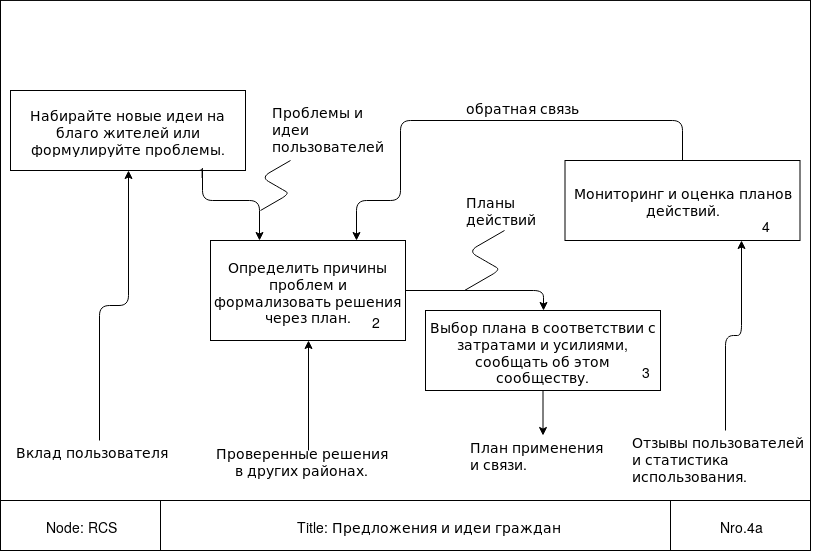
\includegraphics[scale=0.55]{diag4a.png}
  \caption{Структура системы Усовершенствования для соседства}
  \label{image:scheme12}
\end{figure}

\begin{table}[]
\centering
\begin{tabular}{|p{5cm}|p{5cm}|p{5cm}|}
\hline
\multicolumn{3}{|p{15cm}|}{Модульные улучшения для соседства (идеи пользователей)} \\ \hline

 Процесс  & Вход & Выход \\ \hline \hline
Набирайте новые идеи на благо жителей или формулируйте проблемы.& Вклад пользователя &
Проблемы и идеи пользователей\\ \hline
Определить причины проблем и формализовать решения через план. & Проблемы и идеи пользователей.& Планы действий. \\ \hline
Выбор плана в соответствии с затратами и усилиями, сообщать об этом сообществу. & Планы действий.& План применения и связи.\\ \hline
Мониторинг и оценка планов действий. & Отзывы пользователей и статистика использования. & Идеи на благо жителей района.\\ \hline
\end{tabular}
\centering
\caption{Процессы, связанные с улучшением окрестности.}
\centering
\label{tabla:sencilla2}
\end{table}








\chapter{КОНСТРУКТОРСКИЙ РАЗДЕЛ}


\section{Используемые технологии}

Одной из трудных задач является исследование доступных технологий. Каждая технология охватывает широкий спектр знаний, поскольку они являются передовыми технологиями, и в прикладных алгоритмах существует математическая поддержка. Конечно, знание теоретических основ важно, но в то же время необходимо проверить, что есть инструменты, которые служат основой проекта. Мы искали доступные технологии и которые мы сейчас представляем.

ProductionIO \cite{predictionio} выбирается в качестве сервера Machine Learning Server с открытым исходным кодом, поскольку он облегчает задачу разработки приложений на основе Spark и многих других решений для больших данных.

Мы выбираем «Apache PredictionIO» в качестве сервера с открытым исходным кодом для создания прогнозирующего движка, чтобы можно было разработать следующий:

\begin{enumerate}
	\item быстро создавать и развертывать движок в качестве веб-сервиса для производства с настраиваемыми шаблонами;

	\item отвечать на динамические запросы в режиме реального времени после развертывания в качестве веб-службы;

	\item систематически оценивать и настраивать несколько вариантов двигателей;

	\item унифицировать данные с нескольких платформ в пакетном режиме или в режиме реального времени для всесторонней прогностической аналитики;

	\item ускорить моделирование машинного обучения с систематическими процессами и заранее подготовленными оценочными мерами;

	\item библиотеки поддержки обучения и обработки данных, такие как Spark MLLib и OpenNLP;

	\item внедрять модели машинного обучения и плавно включать их в свой двигатель;

	\item упростить управление инфраструктурой данных.
\end{enumerate}

\begin{figure}[h]
  \centering
  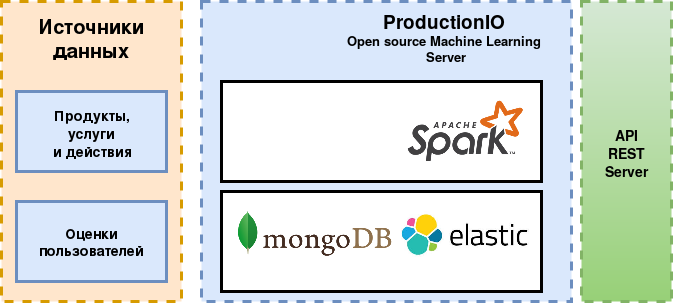
\includegraphics[scale=0.65]{predictionio.png}
  \caption{PredictionIO topology}
  \label{image:alg_timer}
\end{figure}

Apache PredictionIO установлен как полный стековый учебный стек, в комплекте с Apache Spark, MLlib, HBase, Spray и Elasticsearch, который упрощает и ускоряет масштабируемое управление инфраструктурой машинного обучения.

\newpage
\section{Topology}

Наша система рекомендаций разделена на три основных модуля:

\begin{enumerate}
\item Dataset Loader: этот подмодуль загрузит набор данных из Интернета, обработает и сохранит его в наших двух основных хранилищах данных (MongoDB и ElasticSearch).
\item Рекомендательный тренер: все рейтинги, хранящиеся в БД предыдущим модулем, будут использоваться для создания модели совместной совместной работы и предварительного расчета рекомендаций для всех пользователей и продуктов, которые затем будут храниться в MongoDB.
\itemР екомендательный сервер: используя небольшой сервер REST, мы отправим рекомендации для запросов MongoDB и ElasticSearch.
	
\end{enumerate}

Системная топология состоит из распределенной системы обработки информации со следующими задействованными частями: один или несколько экземпляров сервера событий и его механизмы, которые объединяются через API-Rest в центральный API. Центральный API или API «Frontend» - это тот, который взаимодействует с пользователями (веб-браузер, приложение и т. Д.). На первом этапе будет интересна только веб-версия.

\begin{figure}[h]
  \centering
  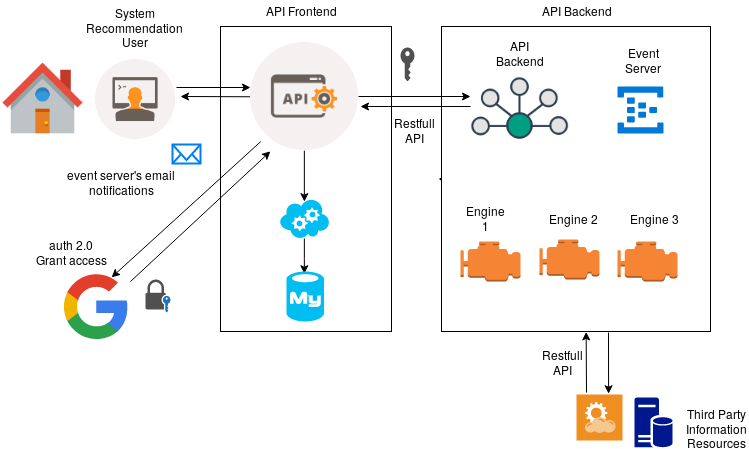
\includegraphics[scale=0.65]{topo2.png}
  \caption{Выбранная топология системы - это микросервисы}
  \label{image:alg_timer2}
\end{figure}


\section{Имплементацион 3 ступени архитектуры}

Три шага в общей архитектуре рекомендательная Системы :
\begin{itemize}
	\item Получение данных
	\item  Предварительно рассчитать
	\item  Получить
\end{itemize}


\textbf{Шаг 1: Проглатывание (Получение данных)}. 
Каждой рекомендуемой системе нужны данные о товарах и пользователях для работы.
\begin{itemize}
	\item Каталог предметов: информация о предметах. Ежедневно / ежечасно обновляется.
	\item Оценки пользователей: неявные или явные оценки генерируются в непрерывном потоке данных.
\end{itemize}


\textbf{Шаг 2: предварительный расчет}.
Рекомендатор Системные недостатки:
\begin{itemize}
	\item Задержка - ключевой фактор в любом сервисе персонализации.
	\item Вычислить рекомендации точно в срок очень дорого и медленно.
\end{itemize}

Наилучшим подходом является предварительный расчет Рекомендаций:
\begin{itemize}
	\item Content Based: современные индексы хранят данные так, что выполнение запросов на поиск выполняется быстро.
	\item Совместная фильтрация: подготовьте модель ALS и предварительно вычислите реквизиты для существующих пользователей и элементов.
\end{itemize}

\textbf{Шаг 3: Получить}. 
Когда запрашиваются рекомендации, просто:
\begin{itemize}
	\item Content Based: создайте запрос, и он будет выполнен индексом.
	\item Collaborative filtering: прочитайте БД для предварительно рассчитанных рекомендаций.
	\item Гибридные подходы: просто попросите несколько источников и объедините результаты.
\end{itemize}



\begin{figure}[h]
  \centering
  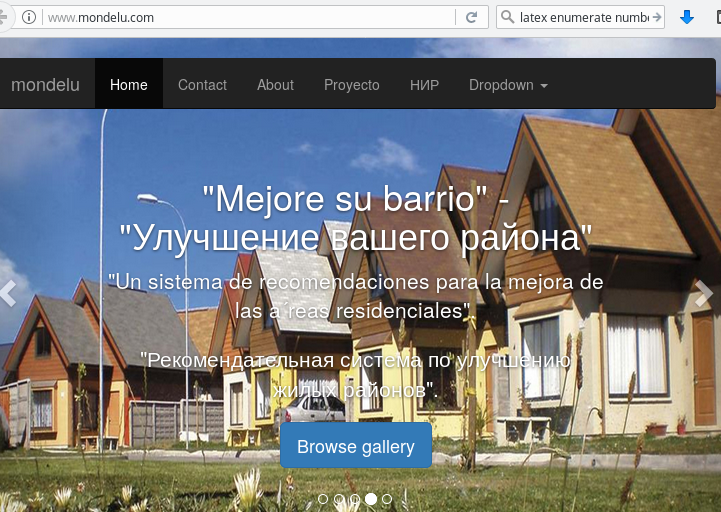
\includegraphics[scale=0.79]{mondelu.png}
  \caption{Test site}
  \label{image:alg_timer3}
\end{figure}

\section{Алгоритмы для рекомендательной системы}

Были выбраны по крайней мере две альтернативы алгоритмов рекомендации. Apache Spark предоставляет различные API-интерфейсы, в этом случае Java API был протестирован в индивидуальной конфигурации на хостинге «DigitalOcean», получив плохие результаты с точки зрения производительности (согласно PredictionIO, требуется минимальная конфигурация 16 ГБ ОЗУ) , В качестве второй альтернативы мы попробуем экземпляр Amazon-EC2 \cite{ec2}(дорогое решение), но только с целью тестирования этих алгоритмов.

\subsection{Алгоритм "K-neighbours" или на основе сходства}

Он будет работать с классом класса «Neighbor», который содержит основной метод программы, который отвечает за вызов остальных классов для выполнения необходимых вычислений. Он также содержит метод для возврата наибольшего идентификационного номера элементов, необходимого для вычисления сходства косинусов.

Он также содержит метод, называемый collectData (), который по пути файла в HDFS читает данные, содержащиеся в нем, и возвращает их в JavaPairRDD, то есть расширение типа ключа / значения RDD, Абстракция искровых объектов. Возвращаемый JavaPairRDD имеет ключевую пару пользователя и в качестве значения содержит элемент и квалификацию (Spark позволяет группировать объекты в одном с классами Tuple2, Tuple3, Tuple4 ...), который связывает пользователя и конкретные элементы, то есть рейтинг, который пользователь дал этому пункту (если он это сделал). Как только эта информация была получена из файла, фильтрация выполняется одним и тем же методом, чтобы ограничить количество пользователей, которые будут участвовать в системе рекомендаций; остальные будут проигнорированы. Это делается для проведения тестов путем изменения количества пользователей и сравнения полученных данных.

После получения сходства между пользователями он выполняет фазу агрегации по рейтингам «соседних» пользователей каждого из них, чтобы получить прогноз рейтинга, который пользователь предоставит каждому элементу.

В MapReduce повторение всех элементов RDD является очень дорогостоящей операцией, поскольку оно поддерживает большой объем данных. Для решения таких проблем, как расчет средних значений пользователей или агрегирование рейтингов, используются восстановительные методы, такие как combByKey, реализация, предоставляемая Spark. Этот метод требует в качестве параметров трех функций: одного из творений, другого дополнения и другого слияния. С первым создается вспомогательный объект указанного типа, при этом к нему добавляются второстепенные элементы, а с третьим объединяются элементы разных объектов (вычисления выполняются параллельно и, следовательно, создается несколько объектов, которые затем они должны собраться).
\subsection{Алгоритм, основанный на тенденциях}

Через класс «Trends», который является основным классом программы, который собирает данные из файла HDFS и управляет вызовом остальным классам. Для получения входных данных он работает так же, как и класс «Соседи» алгоритма, основанного на сходстве.

\subsection{Сравнение альтернатив}

Для этого проекта тестируются по крайней мере два алгоритма, которые позволят в короткие сроки провести дорогостоящие операции. Более конкретно, алгоритм, основанный на «тренде», позволяет проводить миллионы медиа-операций всего за одну секунду.

Сравнивая алгоритм «на основе тенденций» с алгоритмом «K-соседей», оба алгоритма, в которых один имеет более низкую производительность, но лучшую точность данных, а другой, наоборот, должны быть исправлены в ситуации, в которой она предназначена чтобы иметь возможность выбрать один из двух.

С одной стороны, алгоритм, основанный на сходстве или алгоритме соседнего K, имеет очень низкую производительность. Для 8000 пользователей (показатель намного ниже, чем у реальной системы) для выполнения рекомендаций требуется 2 часа. Невозможно использовать его в режиме реального времени, поэтому единственным жизнеспособным выходом для алгоритма, основанного на сходстве, было бы выполнять вычисления в автономном режиме, а затем предлагать их пользователям. Недостатком этого способа предоставления результатов является то, что последние квалификации, которые были сделаны пользователями, не будут учитываться, и хорошие результаты алгоритма с точки зрения уверенности в предсказаниях будут уменьшаться по этой теме.

С другой стороны, алгоритм, основанный на тенденциях, предлагает гораздо лучшие результаты с точки зрения времени. Для системы с 8000 пользователями она рассчитывает прогнозы за 2 минуты, но даже при этом недопустимо ждать пользователя в течение 2 минут (или более) при расчете прогнозов. Он также должен быть выполнен в автономном режиме, но, в отличие от предыдущего алгоритма, он может работать более часто и предлагать более современные данные и, следовательно, уменьшать недостаток, который он имеет с точки зрения точности предсказаний относительно алгоритма, основанного на сходстве.
Выбор того или иного алгоритма будет зависеть от характера системы рекомендаций, которую вы хотите реализовать.

\begin{lstlisting}[language=Scala, caption={Class K Neigborhoods},label=kneigh]
    import org.apache.spark.HashPartitioner;
    import org.apache.spark.SparkConf;
    import org.apache.spark.api.java.JavaPairRDD;
    import org.apache.spark.api.java.JavaSparkContext;
    import org.apache.spark.api.java.function.Function;
    import org.apache.spark.api.java.function.PairFunction;
    import scala.Tuple2;
    import java.util.*;
    public class Neighbours {
        // variables de contexto
        static SparkConf conf;
        static JavaSparkContext sc;

        static public int maxItem (final JavaPairRDD<Integer, Tuple2<Integer, Double>> ratings) {
        return ratings.map(x -> x._2()._1()).top(1).get(0);
        }

        static public JavaPairRDD<Integer, Tuple2<Integer, Double>> collectData(String path, final Integer max){
        return sc.textFile(path)
            .mapToPair(s -> {
                List<String> separated = Arrays.asList(s.split("::"));
                Integer u = Integer.parseInt(separated.get(0)); //usuario
                Integer i = Integer.parseInt(separated.get(1)); // ítem
                Double r = Double.parseDouble(separated.get(2)); // rating
                return new Tuple2(u, new Tuple2(i, r));
            })
            .filter(new Function<Tuple2<Integer, Tuple2<Integer, Double>>, Boolean>() {

            public Boolean call(Tuple2<Integer, Tuple2<Integer, Double>> x) {
                return (x._1().compareTo(max) <= 0); // limitar el número de usuarios
            }   
    });
}


\end{lstlisting}

\newpage
\begin{lstlisting}[language=Scala, caption={Class Trends},label=trends]
    import org.apache.spark.HashPartitioner;
    import org.apache.spark.SparkConf;
    import org.apache.spark.api.java.JavaPairRDD;
    import org.apache.spark.api.java.JavaSparkContext;
    import org.apache.spark.api.java.function.*;
    import scala.Tuple2;
    import java.util.Arrays;
    importjava.util.List;
    public class Trends {
        // variables de contexto
        static SparkConf conf;
        static public JavaSparkContext sc;
        static public JavaPairRDD<Tuple2<Integer,Integer>, Double> collectData(String path, final Integer maxUser){ 
      
            return sc.textFile(path)
                .mapToPair(s -> {
                    List<String> separado = Arrays.asList(s.split("::"));
                    Integer user = Integer.parseInt(separado.get(0));
                    Integer item = Integer.parseInt(separado.get(1));
                    Double r = Double.parseDouble(separado.get(2));
                    return new Tuple2(new Tuple2(user, item), r);
            }).filter(new Function<Tuple2<Tuple2<Integer, Integer>, Double>, Boolean>() {
                public Boolean call(Tuple2<Tuple2<Integer, Integer>, Double> x) {
                    return (x._1()._1().compareTo(maxUser) <= 0); // 1000 usuarios
                }
            });
}
\end{lstlisting}

\newpage

\begin{lstlisting}[language=Scala, caption={Class CosineSimilarity},label=trends]

import org.apache.spark.HashPartitioner;
import org.apache.spark.api.java.JavaPairRDD;
import org.apache.spark.api.java.JavaRDD;
import org.apache.spark.api.java.JavaSparkContext;
import org.apache.spark.api.java.function.PairFunction;
import org.apache.spark.mllib.clustering.VectorWithNorm;
import org.apache.spark.mllib.linalg.BLAS;
import org.apache.spark.mllib.linalg.Vector;
import org.apache.spark.mllib.linalg.Vectors;
import scala.Tuple2;

public class CosineSimilarity {
    final JavaPairRDD<Integer, Tuple2<Integer, Double>> ratings;


    public CosineSimilarity (JavaPairRDD<Integer, Tuple2<Integer, Double>> r) {
        ratings = r.cache();
    }



    public JavaPairRDD<Tuple2<Integer, Integer>, Double> computeSimilarity (final Integer maxItem){
        // entrada: <<usuario1, vector1>, <usuario2, vector2>>
        // salidas: <usuario1, usuario2>, similitudCoseno
        PairFunction<Tuple2<Tuple2<Integer, Vector>, Tuple2<Integer, Vector>>,
            Tuple2<Integer, Integer>, Double> compute =
            (x) -> {
            final Double den1 = (new VectorWithNorm(x._1()._2())).norm();
            final Double den2 = (new VectorWithNorm(x._2()._2())).norm();
            Double num = BLAS.dot(x._2()._2(), x._1()._2());
            return new Tuple2 (new Tuple2(x._1()._1(), x._2()._1()), (num / (den1 * den2)));

            };
    JavaRDD<Tuple2<Integer, Vector>> vectors = ratings
            .groupByKey(new HashPartitioner(7))
            .map(r -> new Tuple2(r._1(), Vectors.sparse(maxItem+1, r._2()))); // <usuario, vectorRatings>
    
    return vectors
            .cartesian(vectors) // <<usuario1, vectorRatings1>, <usuario2, vectorRatings2>>
            .filter(x -> x._1()._1() != x._2()._1()) // user1 != user2
            .mapToPair(compute); // <<user1, user2>, similitud>
    }
}
\end{lstlisting}



\chapter{ТЕХНОЛОГИЧЕСКИЙ РАЗДЕЛ}

\section{Масштабируемость}


Масштабируемость системы, помимо прочего, определяется способностью системы управлять большим объемом данных. Сначала это может показаться не проблемой, но приложения, в основном розничные или розничные, с большим количеством структурированных или неструктурированных данных, имеют тенденцию к экспоненциальному росту.


С этим мы ссылаемся на так называемые BigData \cite{bigdata}, которые относятся к наборам данных или комбинациям наборов данных, размер, сложность которых и скорость роста которых затрудняют сбор, управление, обработку или анализ с использованием традиционных технологий и инструментов, таких как как реляционные базы данных и обычные статистические данные, такие как база данных Mysql \cite{mysql} с использованием языка SQL \cite{sql}, в течение приемлемого времени, поскольку нет смысла иметь ответ через 5 минут.


Поскольку мы не определили, какое количество данных определяет BIGDATA, мы будем искать лучшее решение с наименьшими затратами и обеспечивающее масштабируемость, что, в свою очередь, позволяет нам взаимодействовать с внешними инструментами, такими как ERP, CRM или ad-hoc-системы.

Преимущества BIGDATA можно найти в обширной биографии на эту тему, но поскольку это ключевой момент в рассматриваемой системе, мы подробно описываем:

\begin{itemize}
	\item Быстро для принятия решений Используя соответствующий инструмент и способный объединять разные источники данных, можно сразу анализировать информацию и принимать решения на основе того, что они узнали.


\item Снижение стоимости при использовании сторонних сервисов на основе облака. Хранение большого количества данных в конкретных службах помогает определить более эффективные способы ведения бизнеса.

\item Новые услуги По мере появления новых потребностей с готовностью bigdata предоставление решений становится проще.
\end{itemize}

Теперь ищите лучшее решение для управления большими объемами данных, и что оно доступно и с открытым исходным кодом.

\section{Выберите подходящее вам решение}

Характеристика системы, как мы упоминали в разделе анализа, представляет собой приложение на основе сервисов, которое может быть принято как экземпляр, который распределяется между другими экземплярами.

Первым вариантом является Apache Hadoop, который представляет собой программную среду, которая поддерживает приложения, распространяемые по бесплатной лицензии. Hadoop позволяет приложениям работать с тысячами узлов и большими объемами данных, имеет относительно большое сообщество пользователей и работает под Java.

Второй альтернативой является Apeche Spark, которая идет немного дальше, потому что это кластерное решение для вычислений и обеспечивает интерфейс для программирования полных кластеров с параллелизмом данных и высокой отказоустойчивостью.

Apache Spark - это все-в-кластерное, ориентированное на скорость решение, которое также предоставляет api для Python, R, Java и Scala. Он также имеет встроенную библиотеку для машинного обучения. Теперь сравните Hadoop и Apache Spark:

\begin{enumerate}
	\item \textbf{трудность:} В то время как Apache Spark имеют много операторов высокого уровня, которые делают программирование и поддержку RDD с Hadoop, разработчики должны кодировать каждую операцию, которая делает работу трудно.
	\item \textbf{Простота использования:} Apache Spark может работать в пакетном, интерактивном режиме, режиме машинного обучения или потоковой передачи в одном кластере. Это целый механизм анализа данных, поэтому нет необходимости использовать разные компоненты для каждой потребности. Единая установка Apache Spark охватывает все потребности.
	\item \textbf{Скорость отклика:} Apache Spark - это громоздкий инструмент для кластерных вычислений и запускает приложения со скоростью 100 раз быстрее в памяти и десять быстрее на диске, чем Hadoop. Из-за уменьшения числа циклов R-W на диск и хранения промежуточных данных в памяти Spark позволяет.
Hadoop читает и записывает с диска, с низкой производительностью и низкой скоростью обработки.
	\item \textbf{Отказоустойчивость:} Apache Spark является отказоустойчивым. В результате нет необходимости перезапускать приложение с нуля в случае сбоя. Hadoop MapReduce, как Apache Spark, MapReduce также отказоустойчив, поэтому нет необходимости перезапускать приложение с нуля в случае сбоя.
	\item \textbf{Безопасность:} Apache Spark немного менее безопасен по сравнению с Hadoop, поскольку он поддерживает единственную аутентификацию через аутентификацию с общим секретным паролем. Hadoop MapReduce более безопасен из-за Kerberos, а также поддерживает списки контроля доступа (ACL), которые являются традиционной моделью разрешения файлов.
\end{enumerate}

После этого сравнения ясно, что Apache Spark намного удобнее, если нас не беспокоит сильная безопасность, поэтому мы выбираем Spark, поскольку у него много преимуществ по сравнению с Hadoop\cite{comparison}.


\subsection{Основные модули Spark}

В нашем случае мы попробуем только первый, но посмотрим, что они собой представляют:

Spark SQL - это модуль Spark для обработки структурированных данных. Он обеспечивает абстракцию программирования, называемую DataFrame, а также может выступать в роли распределенного механизма запросов SQL. DataFrame - это распределенный сбор данных, организованный в столбцах.
Концептуально он эквивалентен таблице в реляционной базе данных, но оптимизирован.

GraphX ​​- это новый компонент Spark для графиков и параллельного вычисления графиков. На высоком уровне GraphX ​​расширяет Spark RDD, введя новую абстракцию Графа: прямой мультиграф со свойствами, связанными с каждой вершиной и ссылкой.

Spark Streaming - это расширение ядра API Spark, которое обеспечивает масштабируемую, отказоустойчивую и высокопроизводительную поточную обработку. Он обеспечивает абстракцию высокого уровня, называемую Dstream, которая представляет непрерывное прибытие данных. Внутренне Dstream представлен как последовательность RDD.

Mllib - это масштабируемая библиотека обучения компьютера Spark, состоящая из общих алгоритмов обучения и утилит, включая классификацию, регрессию, кластеризацию, совместную фильтрацию, уменьшение размерности.


\chapter{ЗАКЛЮЧЕНИЕ}


В результате проделанной работы был разработан необходимые инструменты были проанализированы и разработаны для поддержки лучшего управления отзывами пользователей, чтобы обеспечить лучшее управление между жителями района и жителями с городскими властями.


Хотя для обоснования полезности этих инструментов необходимо использовать их пользователями, ясно, что люди предпочитают сотрудничать друг с другом, когда это оправдывает его (лучше жить в сообществе).
Точно так же взаимосвязь между экземплярами системы позволит обменяться отзывами между кварталами и городами по желанию или просто взять лучшие примеры в каждой области.


Хорошее использование обратной связи, в дополнение к полезности, чтобы дать лучшую рекомендацию, помогает улучшить целые процессы, рекомендовать действия или обеспечить лучшее решение проблем. Кроме того, пользовательская обратная связь, когда используется для управления районами или городами, полезна для того, чтобы сделать правительство прозрачным, а граждане больше всего выигрывают.

С использованием приложений, библиотек и программных сред для управления большими объемами данных также возможно, что в будущем он может быть использован для других функций, которые не были обнаружены до сих пор.


Задачи выполнены полностью, а именно:
\begin{itemize}
\item Была разработана полевая работа по изучению существующих компьютерных средств, способствующих развитию городских анклавов.

\item Были проанализированы существующие потребности кварталов, а инструменты были разработаны для поддержки городских анклавов, когда возникла необходимость в улучшении предложения садовых продуктов или домашней краски или путем добавления предложений культурной или развлекательной деятельности при сравнении более развитых районов, чем другие;

\itemТочно так же был изучен способ разработки инструмента поддержки совместной экономики, то есть обмена отзывами пользователя или тех, кто заинтересован в присоединении к этим методологиям работы;

\itemОн был разработан и очерчен инструментом, который поддерживает тип «системы инцидентов», чтобы жители могли информировать правительство о проблемах, которые происходят в окрестностях, чтобы иметь решение;

\itemРазработан и набросал инструмент, который отражает идеи жителей, чтобы улучшить анклавы и что они могут внести свой вклад в план, голосовать за них и представлять правительству;

\itemОни научились использовать некоторые инструменты, которые поддерживают управление BigData, чтобы иметь возможность выполнять указанные ранее и в то же время быть готовыми к новым требованиям;

\end{itemize}


\backmatter

%\Conclusion

В результате выполнения данной курсовой работы был изучен подход динамического написания драйверов под OC Linux, работа с звуковой системой и устройством ввода (гарнитурой).

Исследован сигнал, получаемый от гарнитуры на вход микрофона компьютера. 

Разработана программа, обнаруживающая событие нажатия кнопки гарнитуры и протокол взаимодейсвтия этой программы с модулем ядра. 

Разработан модуль ядра, работающий с клавиатурой, который включает/выключает LED индикаторы клавиатуры. 



\bibliographystyle{gost780u}
\bibliography{index.bib}

\appendix

\end{document}

%%% Local Variables:
%%% mode: latex
%%% TeX-master: t
%%% End:
\grid
